\documentclass[12pt,a4paper]{article}
\usepackage{ctex}         % 中文支持
\renewcommand{\thesection}
{\chinese{section}\hspace{1em}}
\renewcommand{\thesubsection}
{\arabic{section}.\arabic{subsection}}
\usepackage{geometry}
\usepackage{titlesec}
\usepackage{tabularx}
\usepackage{booktabs}
\usepackage{listings}
\usepackage{xcolor}
\usepackage{siunitx}    % 单位格式化（可选）
\usepackage{array}      % 增强列控制
\usepackage{longtable,multirow}
% 设置一级section标题：编号+标题文字整体居中
\titleformat{\section}[block]
{\centering\Large\bfseries}
{\thesection}
{1em}
{}
\usepackage{enumitem}

% 二级subsection保持左对齐（默认）
\titleformat{\subsection}[block]
{\raggedright\large\bfseries}
{\thesubsection}
{0.8em}
{}

\geometry{margin=2.5cm}   % 设置页边距

\usepackage{amsmath,amssymb} % 数学公式
\usepackage{graphicx}        % 插入图片
\usepackage{booktabs}        % 美观表格
\usepackage{float}           % 图片位置控制
\usepackage{listings}
\usepackage{xcolor}
\lstset{
	language=Python,
	basicstyle=\ttfamily\small,
	commentstyle=\color{gray},
	keywordstyle=\color{blue},
	stringstyle=\color{red},
	numbers=left,
	numberstyle=\tiny,
	breaklines=true,
	frame=single
}
\usepackage{hyperref}        % 超链接

\usepackage{listings}
\usepackage{xcolor}

\lstset{
	language=Python,
	basicstyle=\small\ttfamily,
	keywordstyle=\color{blue}\bfseries,
	commentstyle=\color{green!50!black},
	stringstyle=\color{red!80!black},
	numberstyle=\tiny\color{gray},
	stepnumber=1,
	numbersep=5pt,
	showspaces=false,
	showstringspaces=false,
	tabsize=4,
	breaklines=true,
	breakatwhitespace=true,
	frame=single,
	captionpos=b,
	xleftmargin=0.5cm,
	xrightmargin=0.5cm,
}

\title{烟幕干扰弹的投放策略研究}
\date{}  % 不要显示日期



	\begin{document}

	\maketitle
	\begin{abstract}
	现代防空对抗环境下，无人机挂载烟幕干扰弹实施无源遮蔽干扰，能够在不使用硬杀伤武器的条件下保护我方重点目标，具备成本低、部署灵活、效费比高\cite{wei2026}等显著优势。本文围绕烟幕干扰弹投放策略优化问题开展研究\cite{cai2026}，综合分析无人机机动约束、干扰弹重力抛体运动、球状烟幕云团下沉演化、空地导弹匀速直线来袭等多类物理过程，建立完整的三维运动学模型，基于\textbf{线段‑球体几何相交原理}构建有效遮蔽判别准则，以最大化真目标总有效遮蔽时长作为优化目标，依次完成仿真计算、单机单弹优化、\textbf{单机多弹时序规划}、\textbf{多机协同干扰}、\textbf{多机资源分配对抗多枚导弹}共五类问题求解。
	
	首先梳理导弹、无人机、干扰弹、烟幕云团的运动机理，推导各对象随时间变化的位置解析表达式，建立遮蔽时长仿真计算框架，针对问题一给定的无人机飞行速度、投放时刻、起爆延迟条件，代入模型完成有效遮蔽时长定量计算。针对问题二单机单弹优化问题，将无人机飞行方向、飞行速度、投放点、起爆点作为决策变量，结合无人机等高度匀速飞行、速度区间约束、抛体运动约束构建带约束连续优化模型，采用数值寻优算法求解最优投放方案，获得最长遮蔽时间对应的全套参数。对于问题三单机投放3枚干扰弹的场景，额外引入同机投弹时间间隔不少于1s的硬约束，开展\textbf{多弹时序联合优化}，允许多枚烟幕遮蔽窗口不连续，最大化累计遮蔽时长，并输出`result1.xlsx`结果文件。问题四扩展至多机协同作战场景，使用 FY1、FY2、FY3 三架无人机各投放一枚干扰弹，充分利用不同无人机的空间位置优势，通过多组烟幕的时空配合填补遮蔽时间间隙，得到协同干扰投放策略并输出`result2.xlsx`。问题五面向复杂综合对抗场景，五架无人机每架最多可投放3枚干扰弹，同时对抗M1、M2、M3三枚来袭导弹，将问题拆解为弹药资源分配与参数优化两层，既要完成干扰弹药在多架无人机、多枚导弹之间的分配调度，又要对每一枚干扰弹对应的无人机机动、投放、起爆参数进行寻优，最终得到多目标协同干扰方案，输出`result3.xlsx`。
	
	仿真结果表明，本文所建立的运动学与几何判别模型可以准确刻画烟幕干扰作战全过程，不同场景下均能够输出满足全部物理与工程约束的投放参数。本文模型可为无人机烟幕无源干扰作战的任务规划、弹丸投放时序设计提供数学模型支撑与仿真计算手段。

		
		\noindent\textbf{关键词：}\textbf{烟幕干扰弹；运动学模型；有效遮蔽；无人机投放策略；时序优化}
	\end{abstract}
	
	\newpage %摘要结束换页，正文开始
	
	\section{问题重述}
	
	\subsection{问题背景}
	
	烟幕干扰弹主要依靠化学燃烧或者爆炸分散形成烟幕或气溶胶云团，在来袭武器和被保护目标的中间空域形成遮蔽，以此干扰敌方导弹探测\cite{chen2017}，具备成本低廉、效费比突出的优势。随着投放控制技术发展，可以通过时间引信精准控制起爆时刻，实现定点抛撒烟幕干扰弹。

	本次任务采用长续航无人机挂载烟幕干扰弹执行干扰任务。当警戒雷达探测到来袭导弹后，指挥中心立即向无人机下发任务指令，无人机机动至合适空域投放干扰弹，在来袭导弹与我方真目标之间布设烟幕，阻挡导弹对真目标的探测。
	
	\subsection{问题要求}
	
	本题是带多重约束的三维空间运动优化问题。研究对象包含来袭导弹、执行任务无人机、抛射后的烟幕干扰弹、起爆之后动态变化的烟幕云团。问题的核心判定准则：某一时刻，来袭导弹指向真目标的视线线段与处于有效期内的烟幕球体存在交点，则该时刻实现有效遮蔽；优化目标为最大化真目标总的有效遮蔽时长。同时存在大量硬性约束，包括无人机飞行速度范围、等高度匀速直线运动、单机投弹最小时间间隔、烟幕最长有效时间 20 s、烟幕云团仅竖直向下匀速下沉等。
	
	
	根据题目给出的初始位置、装备运动约束、烟幕物理特性，建立数学模型，分别完成以下五个子问题：
	
	\textbf{问题1：}利用无人机 FY1 投放 1 枚烟幕干扰弹干扰 M1 导弹；FY1 以 120 m/s 朝向假目标飞行，受领任务 1.5 s 后投放干扰弹，投放完成后间隔 3.6 s 起爆。计算该条件下烟幕对 M1 的有效遮蔽时长。
	
	\textbf{问题2：}利用无人机 FY1 投放 1 枚烟幕干扰弹实施对 M1 的干扰。确定 FY1 的飞行方向、飞行速度、烟幕干扰弹投放点、起爆点，使真目标有效遮蔽时间尽可能长。
	
	\textbf{问题3：}利用无人机 FY1 投放 3 枚烟幕干扰弹，干扰 M1 导弹，给出完整烟幕干扰弹投放策略，将结果保存至`result1.xlsx`。
	
	\textbf{问题4：}利用 FY1、FY2、FY3 三架无人机，每架各投放 1 枚烟幕干扰弹，对 M1 实施干扰，给出投放策略，将结果保存至`result2.xlsx`。
	
	\textbf{问题5：}使用全部 5 架无人机，每架无人机最多投放 3 枚烟幕干扰弹，同时干扰 M1、M2、M3 三枚来袭导弹，给出投放策略，将结果保存至`result3.xlsx`
	
	
	
	
	\section{问题分析}
	本题五个子问题难度逐级递进：从固定参数下的仿真计算，到单机单弹参数寻优；再扩展到单机多弹的时序优化；之后发展为多机协同对抗单枚导弹；最后为多机多弹药资源分配，同时对抗多枚导弹的高维组合优化问题。问题一为基础仿真模块，后续所有优化子问题均复用问题一建立的遮蔽判别仿真框架
	\subsection{问题一分析}
	\textbf{对于问题一，}	全部运动参数均已经预先给定，不需要进行优化，属于运动仿真与几何判定类问题。
	求解分为四步：\textbf{首先}根据无人机初始位置、飞行速度、航向，计算\(t=1.5\ \text{s}\)时刻干扰弹投放点的三维坐标；\textbf{其次}建立干扰弹脱离无人机后的重力抛体运动方程，结合 3.6 s 起爆延迟，求解干扰弹起爆时刻对应的起爆点坐标；\textbf{然后}分别建立导弹 M1 位置随时间变化的运动方程、烟幕云团球心随时间变化的位置方程；\textbf{最后}在导弹飞抵假目标的全部时间区间内逐时刻判断：M1 到真目标的视线线段是否和处于有效期的烟幕球体相交；统计满足遮蔽条件的总时长，即为有效遮蔽时长。
	
	该问搭建的仿真与几何判别模块，是后面所有优化问题的基础
	
	
	\subsection{问题二分析}
	\textbf{对于问题二，}本问属于单机单弹的连续优化问题。决策变量为无人机飞行方向、飞行速度、干扰弹投放时刻、起爆延迟时间。
	约束条件包括：无人机飞行高度保持初始高度不变；飞行速度\(70\le v \le140\ \text{m/s}\)；干扰弹投放之后仅受重力做抛体运动；烟幕起爆后有效时间上限为 20 s。目标函数为有效遮蔽时长最大化。

	该问可以采用数值寻优算法：遍历或者智能算法更新决策变量，调用问题一的仿真遮蔽时长计算模型，不断计算对应目标函数，搜索得到遮蔽时间最大的一组参数，输出无人机飞行参数、投放点、起爆点坐标。
	
	\subsection{问题三分析}
	\textbf{对于问题三，}本问为单机多弹时序优化问题，在问题二单弹模型基础上增加约束条件：同一架无人机投放两枚干扰弹的投放时刻之差不得小于 1 s，总共投放 3 枚干扰弹。每一枚干扰弹均包含投放时刻、起爆延迟两组决策变量；多枚烟幕的遮蔽时间允许叠加、允许不连续。优化目标为 3 枚干扰弹贡献的总有效遮蔽时长最大化。
	
	在满足无人机运动约束、投弹间隔约束前提下，对三枚干扰弹的投放时序、起爆时刻进行联合寻优，得到完整投放方案，输出至`result1.xlsx`。
	
	\subsection{问题四分析}
	\textbf{对于问题四，}本问属于多无人机协同干扰单目标的优化问题。FY1、FY2、FY3 三架无人机各自投放一枚干扰弹对抗 M1 导弹。每一架无人机拥有独立的飞行方向、飞行速度、投放时刻、起爆延迟决策变量；不同无人机之间不存在投弹时间间隔约束。
	
	优化思路：各无人机独立规划机动、投放与起爆时刻，通过多团烟幕在时间维度上相互衔接，填补遮蔽时间空白，最大化总的有效遮蔽时长，将全部无人机的策略输出保存为`result2.xlsx`。
	\subsection{问题五分析}
	\textbf{对于问题五，}本问为全场景综合资源分配优化，难度最高。5 架无人机，每架最多投放 3 枚干扰弹，需要同时对抗 M1、M2、M3 三枚来袭导弹。
	该问题包含两层优化：第一层是\textbf{资源分配}，确定每架无人机投放多少枚干扰弹，每一枚干扰弹分配用于对抗哪一枚导弹；第二层为每一枚干扰弹对应的无人机机动、投放、起爆\textbf{参数优化}。需要同时满足无人机飞行约束、单机投弹间隔约束、单枚烟幕最长 20 s 有效时间约束。目标为三枚导弹对应的总有效遮蔽时长尽可能大，属于高维组合优化问题。求解完成后输出全部投放策略至`result3.xlsx`。
	
	\section{模型假设}
	为构建可求解的数学模型，结合赛题给出物理条件，忽略次要影响因素，做出如下合理假设：
	
	(1)指挥中心雷达发现导弹后，指令可以瞬间下发至无人机；无人机受领任务后可以瞬时完成航向调整，不存在转向机动时间，通信无时间延迟。
	
	(2)来袭 M1、M2、M3 导弹视作质点，始终以 300 m/s 做匀速直线运动，飞行方向始终指向假目标；导弹不会受烟幕干扰改变飞行轨迹。
	
	(3)无人机受领任务后保持初始高度不变，进行匀速直线运动；飞行速度严格处于\(70\sim140\ \text{m/s}\)，航向、速度确定后全程不再更改。
	
	(4)烟幕干扰弹脱离无人机瞬间，初速度与无人机瞬时速度完全相同；脱离之后仅受重力作用，忽略空气阻力、风力，遵循三维抛体运动规律。
	
	(5)干扰弹起爆瞬时立刻生成标准球形烟幕云团\cite{wu2016}，不存在起爆过渡过程；云团球心水平坐标固定不变，仅以3m/s竖直向下匀速下沉；忽略风场、湍流带来的云团形变、水平漂移。
	
	(6)烟幕云团起爆之后仅20s内具备遮蔽效果，20s后直接失去遮蔽能力，不考虑浓度渐变衰减；有效遮蔽区域严格为以云团球心为中心，半径10m的球体。
	
	(7)遮蔽判定仅采用几何相交准则：某时刻来袭导弹位置指向真目标的视线线段，与有效烟幕球体存在交点，则判定该时刻实现有效遮蔽；忽略光衍射、散射等复杂光学效应。
	
	(8)作战空域开阔，不存在地形、建筑遮挡，导弹指向真目标的视线不受障碍物阻挡。
	
	(9)仅同一架无人机投放干扰弹存在投放时刻至少间隔1s的约束，不同无人机之间投弹时刻不受该时间间隔限制。
	
	(10)无人机、干扰弹、导弹全部抽象为空间质点，不考虑自身实体几何尺寸；仅烟幕云团保留球体几何特征。
	
	(11)保护目标判定以真目标本体为准，只要导弹指向真目标的视线被烟幕球体遮挡，即完成干扰任务。
	
	\section{符号说明}
	\begin{table}[H]
		\centering
		\begin{tabular}{ccc}
			\toprule
			符号 & 含义 & 单位 \\
			\midrule
			$t=0$ & 雷达发现时刻，计时起点 & s \\
			$t_d$ & 投放时刻，无人机释放烟幕弹的时刻 & s \\
			$t_b$ & 起爆时刻，烟幕弹爆炸并形成云团的时刻 & s \\
			$D$ & 投放点，烟幕弹脱离 FY1 的空间位置 & m \\
			$C_b$ & 起爆点，烟幕弹起爆瞬间的空间位置 & m \\
			$C(t)$ & 云团中心，起爆后球状烟幕云团中心 & m \\
			$R$ & 有效半径，云团可提供有效遮蔽的半径 & m \\
			$w$ & 云团下沉速度，起爆后云团中心竖直下降速度 & m/s \\
			$L(\lambda,t)$ & 视线线段，导弹位置到真目标代表点的线段 & m \\
			$\lambda^*$ & 投影参数，云团中心到视线直线的正交投影参数 & 无量纲 \\
			$d(t)$ & 最短距离，云团中心到视线线段的距离 & m \\
			$T_\mathrm{eff}$ & 有效遮蔽时长，$d(t)\le R$ 且在云团寿命内的总时长 & s \\
			$P$ & 真目标代表点，用于视线判定的目标中心点 $(0,200,5)$ & m \\
			$\bar{\lambda}$ & 截断后的投影参数，限定在线段范围之内 & 无量纲 \\
			$D$ & 假目标点，导弹M1的瞄准点，坐标原点$(0,0,0)$ & m \\
			$T_0$ & 真目标底面圆心，圆柱真目标底面圆心$(0,200,0)$ & m \\
			$T_c$ & 真目标几何中心，圆柱真目标几何中心$(0,200,5)$ & m \\
			$M(t)$ & 导弹位置，M1在时刻$t$的三维位置 & m \\
			$t_M$ & 导弹命中时间，M1到达假目标点$D$的时间 & s \\
			$F(t)$ & 无人机位置，FY1在时刻$t$的位置 & m \\
			$\psi$ & 航向角，FY1水平速度方向与$x$轴夹角 & $\mathrm{rad}/^\circ$ \\
			$v$ & 无人机速度，FY1水平匀速飞行速度 & m/s \\
			$t_r$ & 投放时刻，烟幕弹脱离FY1的时刻 & s\\
			\bottomrule
		\end{tabular}
		\label{tab:symbol}
	\end{table}

	\newpage	
	\section{问题一模型的建立与求解}
	\subsection{坐标系的建立}
	分析烟幕干扰的遮挡效果，关键是判断导弹指向真目标的视线是否被烟幕阻挡。为定量描述假目标、真目标、各枚导弹与无人机的空间位置关系，建立三维直角坐标系 \(O‑XYZ\)，取假目标所在位置为坐标原点 O；三个坐标轴的单位均为米（\(\mathrm{m}\)）：X轴、Y轴在水平面内，Z轴竖直向上。题目给出的各实体初始坐标均可直接在该坐标系下表示：3 枚来袭导弹 M1、M2、M3 与 5 架无人机 FY1～FY5 为运动载体；真目标为底面圆心位于 \((0,200,0)\)、底面半径7m、高度10m的圆柱体；烟幕可视为半径10m的球体。通过该统一坐标系，可以计算任意时刻导弹位置、无人机可达区域、导弹真目标视线方程，并判断视线是否与烟幕球相交，从而完成遮蔽时长的定量计算。如图 1 所示
	
	\begin{figure}[H]
	\centering
	
\includegraphics[width=0.7\linewidth]{C:/Users/HYX/OneDrive/Desktop/coordinate_system}
	\caption{题目给定三维坐标系}
	\label{fig:coordinatesystem}	
	\end{figure}
	
	
	
	
	将雷达发现时刻作为计时起点 $t=0$。已知导弹M1、无人机FY1的初始位置与运动状态；无人机接收指令后延迟 $1.5\ \mathrm{s}$ 执行投放，烟幕弹投放后引信延迟 $3.6\ \mathrm{s}$ 起爆。起爆后形成球形烟幕云团，云团具有固定有效半径与有限有效寿命，云团中心存在恒定竖直下沉速度。真目标为圆柱形，底面圆心为 $(0,200,0)\ \mathrm{m}$，半径 $7\ \mathrm{m}$，高度 $10\ \mathrm{m}$。
	
	待求解量包括：烟幕弹起爆时刻、起爆点位置、有效遮蔽时间区间以及总有效遮蔽时长。模型基础参数如表~\ref{tab:para_base}所示。
	
	\begin{table}[htbp]
		\centering
		\caption{模型基础参数}
		\label{tab:para_base}
		\begin{tabular}{l r}
			\toprule
			物理量 & 数值 \\
			\midrule
			导弹M1初始位置 & $(20000,0,2000)\ \mathrm{m}$ \\
			导弹飞行速度 & $300\ \mathrm{m/s}$ \\
			FY1初始位置 & $(17800,0,1800)\ \mathrm{m}$ \\
			FY1飞行速度 & $120\ \mathrm{m/s}$，朝向假目标原点 \\
			接令后投放延迟 & $1.5\ \mathrm{s}$ \\
			投放后起爆引信延迟 & $3.6\ \mathrm{s}$ \\
			重力加速度 & $g=9.8\ \mathrm{m/s^2}$ \\
			烟幕云团有效半径 & $R=10\ \mathrm{m}$ \\
			云团下沉速度 & $w=3\ \mathrm{m/s}$ \\
			云团有效寿命 & 起爆后 $20\ \mathrm{s}$ \\
			真目标底面圆心 & $(0,200,0)\ \mathrm{m}$，半径 $7\ \mathrm{m}$，高度 $10\ \mathrm{m}$ \\
			\bottomrule
		\end{tabular}
	\end{table}
	

	
	\subsection{运动学模型}

	\textbf{导弹运动模型：}
	
	导弹以300m/s速度直线飞向假目标原点，写出导弹随时间变化位置$\boldsymbol{P}_M(t)$。
	导弹在时刻 $t$ 的位置为 $\boldsymbol{M}(t)$，真目标为一圆柱体。为简化判定，首先以圆柱体的几何中心 $\boldsymbol{P}=(0,200,5)$ 作为目标代表点进行视线判定（更精确的圆柱表面多点判定将在问题二及后续问题中引入）。
	
	导弹指向目标代表点的视线为一条有限线段，其参数化表示为
	\[
	\boldsymbol{L}(\lambda,t)=\boldsymbol{M}(t)+\lambda\cdot \bigl[\boldsymbol{P}-\boldsymbol{M}(t)\bigr],\quad 0\le \lambda\le 1.
	\]
	其中 $\lambda$ 为参数，$\lambda=0$ 对应导弹位置，$\lambda=1$ 对应目标位置。
	
	\subsection{点到线段最短距离的计算}
	烟幕云团球心 $\boldsymbol{C}(t)$ 到视线无限直线的正交投影参数为
	\[
	\lambda^{*}(t)=\frac{\bigl[\boldsymbol{C}(t)-\boldsymbol{M}(t)\bigr]\cdot \bigl[\boldsymbol{P}-\boldsymbol{M}(t)\bigr]}{\bigl\|\boldsymbol{P}-\boldsymbol{M}(t)\bigr\|^{2}}.
	\]
	
	由于视线是有限线段而非无限直线，需将投影参数截断至线段范围 $[0,1]$ 内：
	\[
	\widetilde{\lambda}(t)=\min\bigl(1,\max\bigl(0,\lambda^{*}(t)\bigr)\bigr).
	\]
	
	则烟幕球心到视线线段的最短距离为
	\[
	d(t)=\Bigl\|\boldsymbol{C}(t)-\boldsymbol{M}(t)-\widetilde{\lambda}(t)\cdot \bigl[\boldsymbol{P}-\boldsymbol{M}(t)\bigr]\Bigr\|.
	\]
	
	当且仅当该最短距离不大于烟幕有效半径 $R=10\,\text{m}$ 时，烟幕球体与视线线段存在交点，即该时刻实现有效遮蔽。
	
	
	FY1沿 $-x$ 方向等高度飞行，单位方向向量 $\boldsymbol e_F=(-1,0,0)$。投放时刻 $t_d=1.5\ \mathrm{s}$，投放点位置：
	\[
	\boldsymbol D=\boldsymbol F_0+120 t_d \boldsymbol e_F \approx (17620.00,0,1800)\ \mathrm{m}.
	\]
	引信延迟 $\tau_b=3.6\ \mathrm{s}$，起爆时刻：
	\[
	t_b = t_d + \tau_b = 5.1\ \mathrm{s}.
	\]
	烟幕弹起爆点：
	\[
	\boldsymbol C_b=\boldsymbol D+120\tau_b \boldsymbol e_F+\left(0,0,-\frac12 g \tau_b^2\right)
	\approx(17188.0,0,1736.496)\ \mathrm{m}.
	\]
	令 $s = t-t_b$ 为起爆后经过的时间，则起爆后云团中心位置为
	\[
	\boldsymbol C(t)=\boldsymbol C_b+(0,0,-3s),\qquad 0\le s \le 20.
	\]
	\textbf{无人机运动模型：}
	
	无人机 FY1 在 $t=0$ 时刻位于 $\boldsymbol{F}_0=(17800,\,0,\,1800)$，保持飞行高度 $z=1800\,\text{m}$ 不变，以速度 $v_U$ 沿水平方向做匀速直线运动。设无人机水平飞行的单位方向向量为 $\boldsymbol{e}_d=(\cos\psi,\,\sin\psi,\,0)$，其中 $\psi$ 为航向角（从 $X$ 轴正向逆时针量取），则无人机在任意时刻 $t$ 的位置为
	\[
	\boldsymbol{F}(t)=\boldsymbol{F}_0 + v_U\cdot \boldsymbol{e}_d\cdot t=\bigl(17800 + v_U\cos\psi\cdot t,\; v_U\sin\psi\cdot t,\; 1800\bigr).
	\]
	满足$\|\boldsymbol{e}_d\|=1$；$70\le v_U \le 140$。
	
	\textbf{干扰弹抛体运动模型：}
	
	烟幕干扰弹在投放时刻 $t_d$ 从无人机挂载点脱离，脱离瞬间的初速度与无人机瞬时速度完全相同，即水平分速度为 $(v_U \cos\psi,\; v_U \sin\psi,\; 0)$，竖直分速度为 $0$。脱离后，干扰弹仅受重力作用，忽略空气阻力，遵循三维抛体运动规律。
	
	
	设投放时刻$t_\text{drop}$，投放点$\boldsymbol{P}_\text{drop}=\boldsymbol{P}_U(t_\text{drop})$；干扰弹脱离后只受重力，$z$方向重力加速度$g$。
	\[
	\begin{cases}
		x(t) = x_\text{drop} + v_{Ux}(t-t_\text{drop})\\
		y(t) = y_\text{drop} + v_{Uy}(t-t_\text{drop})\\
		z(t) = z_\text{drop} + v_{Uz}(t-t_\text{drop})-\dfrac12 g(t-t_\text{drop})^2
	\end{cases}
	\]
	起爆时刻$t_\text{det}$，代入得到起爆点坐标$\boldsymbol{P}_\text{det}=\big(x(t_\text{det}),y(t_\text{det}),z(t_\text{det})\big)$。
	
	
	\textbf{视线遮蔽判定模型：}
	
	真目标代表点 $\boldsymbol P=(0,200,5)$。导弹—目标视线线段参数形式：
	\[
	\boldsymbol L(\lambda,t)=\boldsymbol M(t)+\lambda\big[\boldsymbol P-\boldsymbol M(t)\big],\quad 0\le \lambda \le 1.
	\]
	云团中心向视线无限直线的投影参数：
	\[
	\lambda^{*}(t)=
	\frac{\big[\boldsymbol C(t)-\boldsymbol M(t)\big]\cdot \big[\boldsymbol P-\boldsymbol M(t)\big]}
	{\|\boldsymbol P-\boldsymbol M(t)\|^2}.
	\]
	将投影参数截断至线段范围：$\bar{\lambda}=\min\big(1,\max(0,\lambda^{*})\big)$。云团中心到视线线段最短距离：
	\[
	d(t)=\left\|\boldsymbol C(t)-\boldsymbol M(t)-\bar{\lambda}(t)\big[\boldsymbol P-\boldsymbol M(t)\big]\right\|.
	\]
	构造有效遮蔽指示函数
	\[
	I(t)=
	\boldsymbol 1\big\{t_b\le t\le t_b+20,\ d(t)\le R\big\}.
	\]
	总有效遮蔽时长通过积分得到：
	\[
	T_{\mathrm{eff}}=\int_{t_b}^{t_b+20} I(t)\,\mathrm{d}t.
	\]
		
	\textbf{烟幕云团时空演化模型：}
	
	干扰弹在起爆瞬间立刻生成球形烟幕云团，云团球心初始位置即为起爆点 $\boldsymbol{C}_b$。起爆后，云团球心的水平坐标（$X$、$Y$ 方向）保持不变，仅 $Z$ 坐标以恒定速度 $w=3\,\text{m/s}$ 竖直向下匀速下沉。设 $s=t-t_b$ 为起爆后经过的时间（$0\le s\le 20\,\text{s}$），则云团球心在时刻 $t$ 的位置为
	\[
	\boldsymbol{C}(t)=\boldsymbol{C}_b+
	\begin{pmatrix}
		0\\
		0\\
		-w\cdot (t-t_b)
	\end{pmatrix}
	=
	\begin{pmatrix}
		x_{C_b}\\
		y_{C_b}\\
		z_{C_b}-3(t-t_b)
	\end{pmatrix},\quad t_b\le t\le t_b+20.
	\]
	
	当 $t<t_b$ 时云团尚未形成，当 $t>t_b+20$ 时云团失效，这两种情况下云团均不具备遮蔽能力。
	

	
	\subsection{模型求解结果}
	
	导弹在时刻 $t$ 的位置为 $\boldsymbol{M}(t)$，真目标为一圆柱体。为简化判定，首先以圆柱体的几何中心 $\boldsymbol{P}=(0,200,5)$ 作为目标代表点进行视线判定。
	
	导弹指向目标代表点的视线为一条有限线段，其参数化表示为
	\[
	\boldsymbol{L}(\lambda,t)=\boldsymbol{M}(t)+\lambda\cdot \bigl[\boldsymbol{P}-\boldsymbol{M}(t)\bigr],\quad 0\le \lambda\le 1.
	\]
	其中 $\lambda$ 为参数，$\lambda=0$ 对应导弹位置，$\lambda=1$ 对应目标位置。
	
	
	烟幕云团球心 $\boldsymbol{C}(t)$ 到视线无限直线的正交投影参数为
	\[
	\lambda^{*}(t)=\frac{\bigl[\boldsymbol{C}(t)-\boldsymbol{M}(t)\bigr]\cdot \bigl[\boldsymbol{P}-\boldsymbol{M}(t)\bigr]}{\bigl\|\boldsymbol{P}-\boldsymbol{M}(t)\bigr\|^{2}}.
	\]
	
	由于视线是有限线段而非无限直线，需将投影参数截断至线段范围 $[0,1]$ 内：
	\[
	\widetilde{\lambda}(t)=\min\bigl(1,\max\bigl(0,\lambda^{*}(t)\bigr)\bigr).
	\]
	
	则烟幕球心到视线线段的最短距离为
	\[
	d(t)=\Bigl\|\boldsymbol{C}(t)-\boldsymbol{M}(t)-\widetilde{\lambda}(t)\cdot \bigl[\boldsymbol{P}-\boldsymbol{M}(t)\bigr]\Bigr\|.
	\]
	
	当且仅当该最短距离不大于烟幕有效半径 $R=10\,\text{m}$ 时，烟幕球体与视线线段存在交点，即该时刻实现有效遮蔽。
	
	导弹在时刻 $t$ 的位置为 $\boldsymbol{M}(t)$，真目标为一圆柱体。为简化判定，首先以圆柱体的几何中心 $\boldsymbol{P}=(0,200,5)$ 作为目标代表点进行视线判定（更精确的圆柱表面多点判定将在问题二及后续问题中引入）。
	
	导弹指向目标代表点的视线为一条有限线段，其参数化表示为
	\[
	\boldsymbol{L}(\lambda,t)=\boldsymbol{M}(t)+\lambda\cdot \bigl[\boldsymbol{P}-\boldsymbol{M}(t)\bigr],\quad 0\le \lambda\le 1.
	\]
	其中 $\lambda$ 为参数，$\lambda=0$ 对应导弹位置，$\lambda=1$ 对应目标位置。
	

	烟幕云团球心 $\boldsymbol{C}(t)$ 到视线无限直线的正交投影参数为
	\[
	\lambda^{*}(t)=\frac{\bigl[\boldsymbol{C}(t)-\boldsymbol{M}(t)\bigr]\cdot \bigl[\boldsymbol{P}-\boldsymbol{M}(t)\bigr]}{\bigl\|\boldsymbol{P}-\boldsymbol{M}(t)\bigr\|^{2}}.
	\]
	
	由于视线是有限线段而非无限直线，需将投影参数截断至线段范围 $[0,1]$ 内：
	\[
	\widetilde{\lambda}(t)=\min\bigl(1,\max\bigl(0,\lambda^{*}(t)\bigr)\bigr).
	\]
	
	则烟幕球心到视线线段的最短距离为
	\[
	d(t)=\Bigl\|\boldsymbol{C}(t)-\boldsymbol{M}(t)-\widetilde{\lambda}(t)\cdot \bigl[\boldsymbol{P}-\boldsymbol{M}(t)\bigr]\Bigr\|.
	\]
	
	当且仅当该最短距离不大于烟幕有效半径 $R=10\,\text{m}$ 时，烟幕球体与视线线段存在交点，即该时刻实现有效遮蔽。
	
	
	采用时间网格扫描结合二分法求根。在区间 $[t_b,t_b+20]$ 上构造离散时间网格，逐时刻计算导弹位置、云团中心位置、投影参数以及最短距离 $d(t)$，定位 $d(t)-R$ 发生符号变化的区间；再利用二分法精确求解遮蔽开始与结束时刻 $t_1$、$t_2$，最终得到有效遮蔽总时长 $T_{\mathrm{eff}}=t_2-t_1$。
	
	
	经数值求解得到：起爆时刻 $t_b=5.100\ \mathrm{s}$；有效遮蔽起始时刻 $t_1=8.013\ \mathrm{s}$，结束时刻 $t_2=9.448\ \mathrm{s}$，有效遮蔽时间区间为 $[8.013,9.448]\ \mathrm{s}$。总有效遮蔽时长
	\[
	\boxed{T_{\mathrm{eff}}\approx 1.435\ \mathrm{s}\approx 1.44\ \mathrm{s}.}
	\]
	
	如下图
	
\begin{figure}[H]
	\centering
	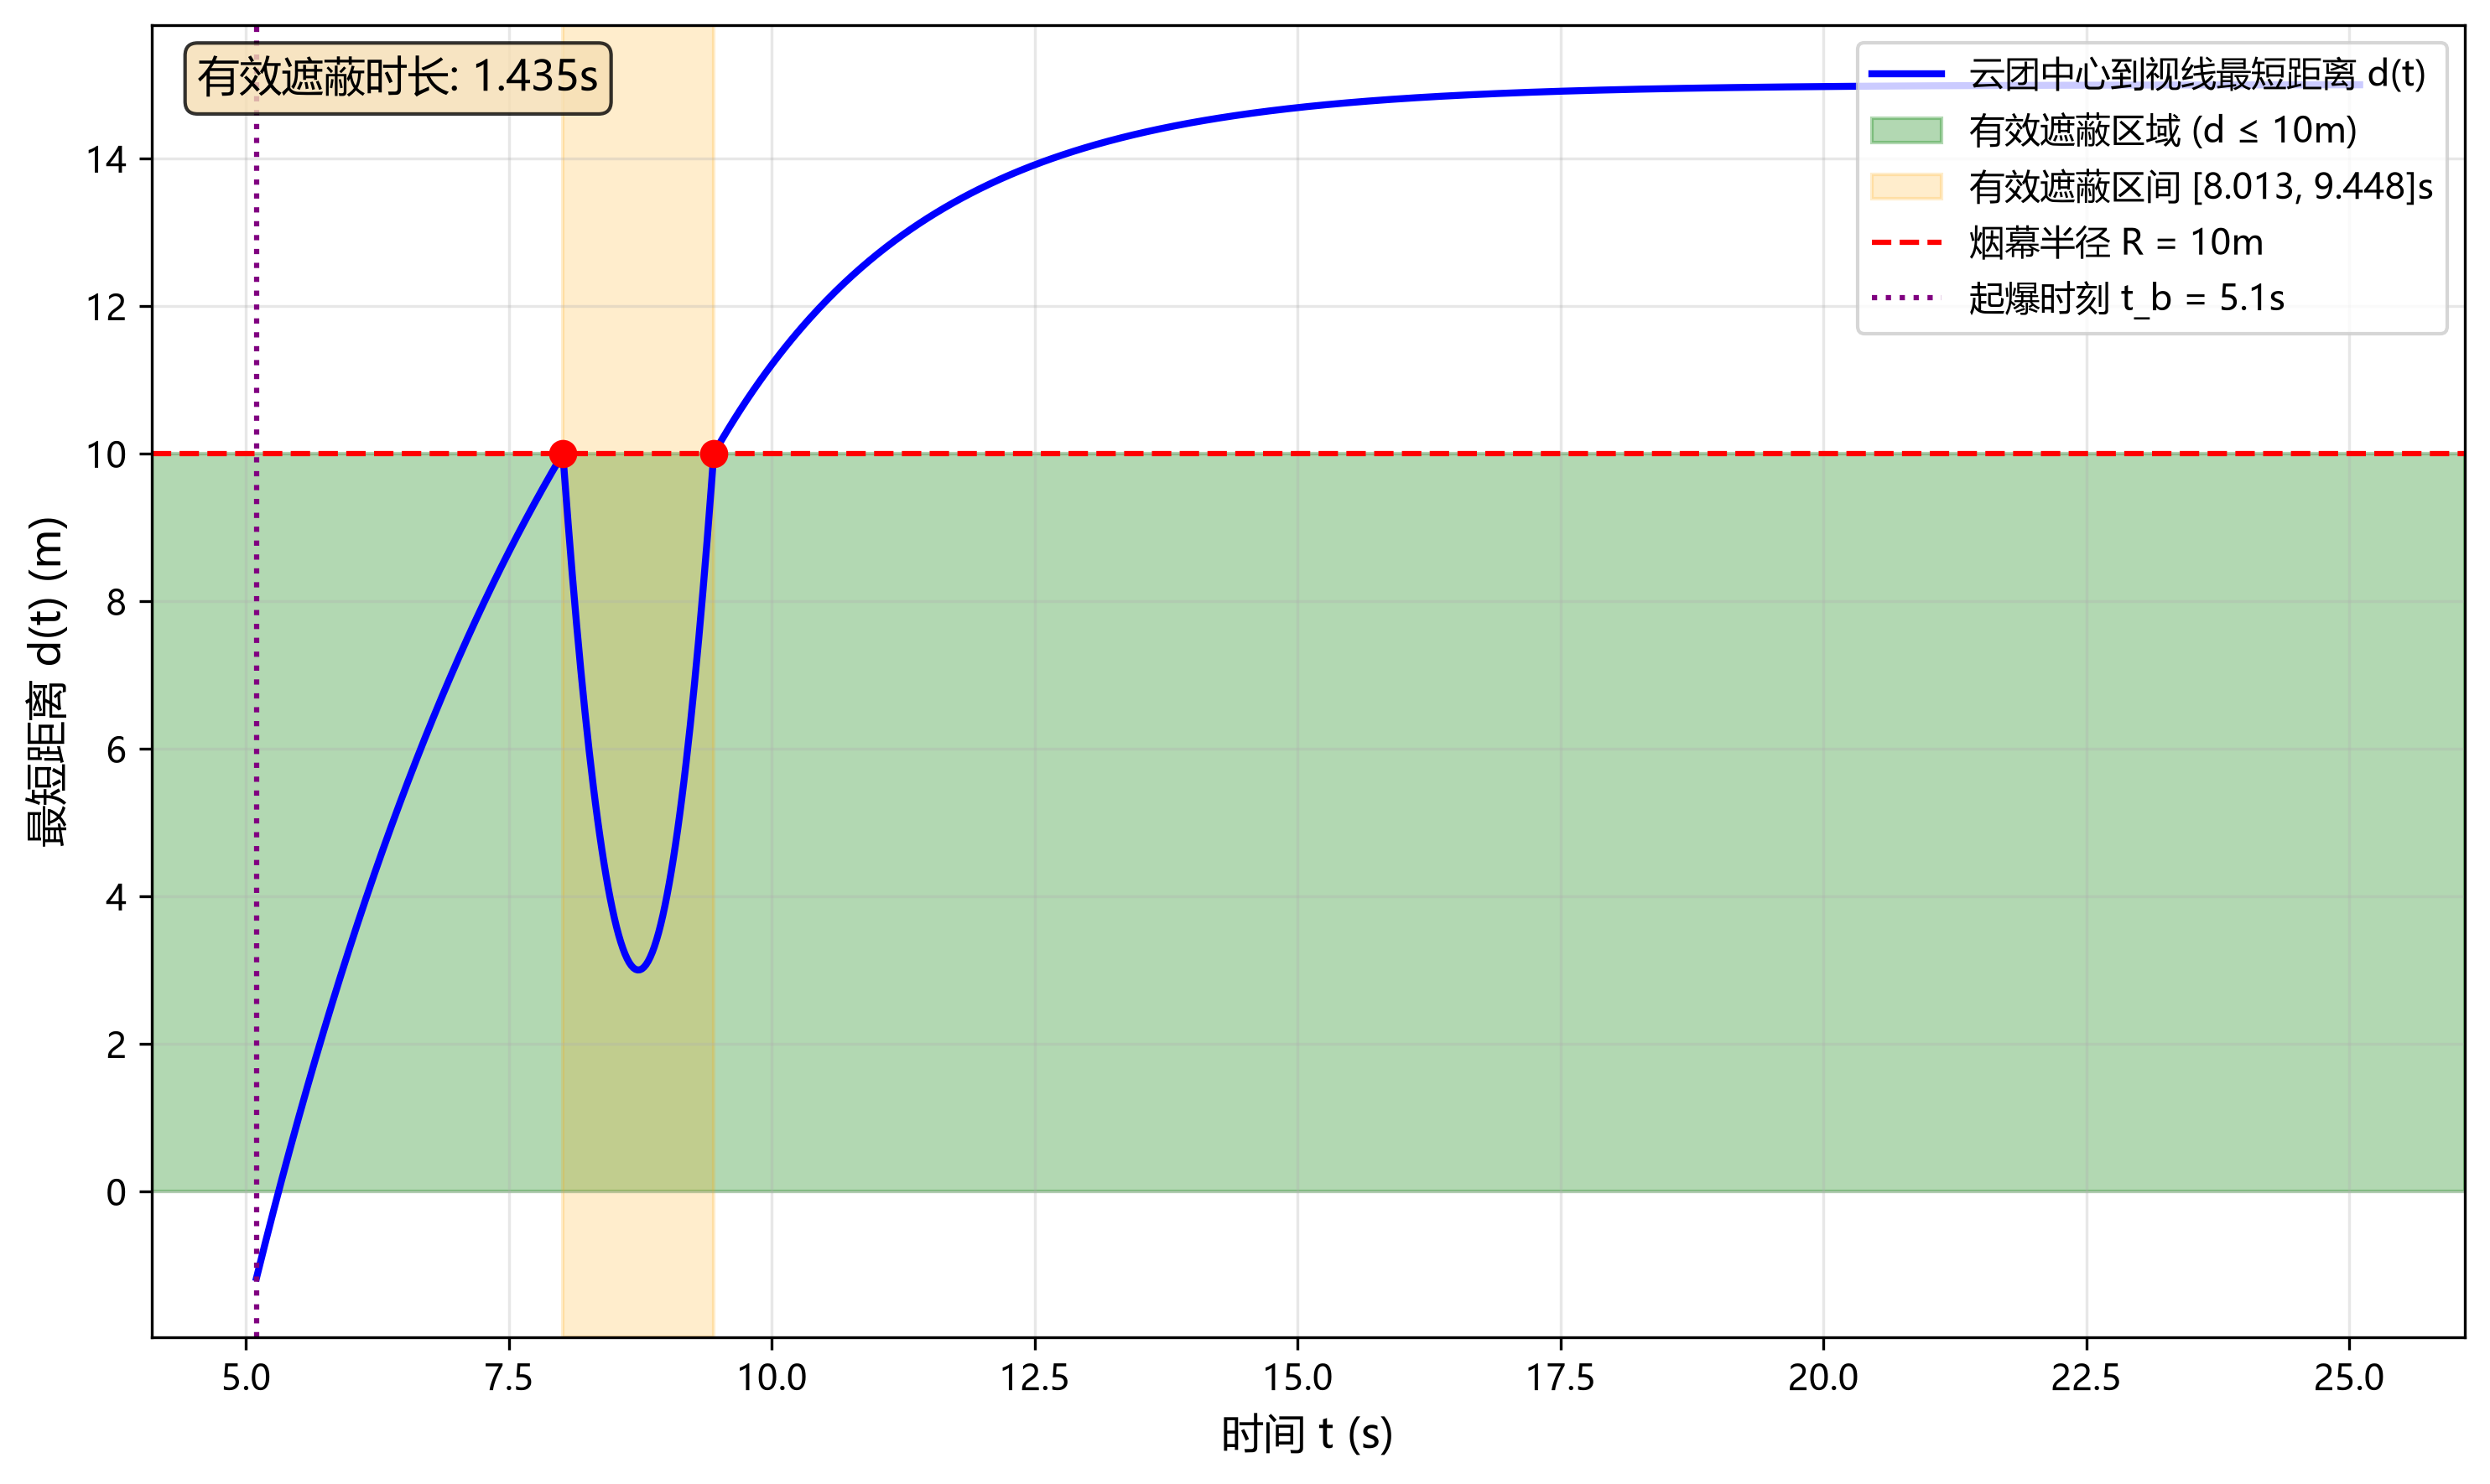
\includegraphics[width=0.7\linewidth]{fig2_q1_distance_curve}
	\caption{烟幕云团中心到视线线段最短距离随时间变化}
	\label{fig:fig2q1distancecurve}
\end{figure}
	


	
	\section{问题二模型的建立与求解}
	
	问题二取消问题一中对无人机FY1航向与飞行速度的固定设定，要求FY1投放一枚烟幕干扰弹对抗来袭导弹M1。在无人机飞行速度取值范围$70\sim 140\ \mathrm{m/s}$的约束下，优化无人机飞行方向、飞行速度、烟幕弹投放时刻以及起爆延迟，尽可能延长烟幕对圆柱形真目标的有效遮蔽时长，输出最优飞行与投放参数、投放点、起爆点以及有效遮蔽时间区间。

	导弹M1初始位置为$(20000,0,2000)\ \mathrm{m}$，以$300\ \mathrm{m/s}$的速度匀速飞向作为假目标的坐标原点。FY1初始位置为$(17800,0,1800)\ \mathrm{m}$，飞行过程中保持高度不变，做水平匀速直线运动。烟幕弹脱离无人机后仅受重力作用；起爆瞬间形成半径$10\ \mathrm{m}$的球形烟幕云团，云团中心以$3\ \mathrm{m/s}$的速度竖直下沉，起爆后$20\ \mathrm{s}$内具备有效遮蔽能力。待保护的真目标为圆柱体，底面圆心坐标$(0,200,0)\ \mathrm{m}$，底面半径$7\ \mathrm{m}$，高度$10\ \mathrm{m}$。
	
	
	
	\textbf{运动学模型：}
	导弹M1朝向假目标原点$\boldsymbol D=(0,0,0)$飞行，导弹至原点的距离以及导弹命中假目标的时刻为
	\[
	L_M=\|\boldsymbol D-\boldsymbol M_0\|=20099.75\ \mathrm{m},\qquad t_M=\frac{L_M}{300}=67.0\ \mathrm{s}.
	\]
	导弹飞行的单位方向向量
	\[
	\boldsymbol e_M=\frac{\boldsymbol D-\boldsymbol M_0}{\|\boldsymbol D-\boldsymbol M_0\|}=(-0.995037,\ 0,\ -0.099504).
	\]
	任意时刻导弹的空间位置
	\[
	\boldsymbol M(t)=\boldsymbol M_0+300t\boldsymbol e_M,\quad 0\le t\le t_M.
	\]
	
	记FY1的水平航向角为$\psi$，飞行速度为$v$，则无人机水平飞行单位方向向量为
	\[
	\boldsymbol e_F=(\cos\psi,\sin\psi,0), \qquad 70 \le v \le 140,
	\]
	FY1随时间变化的位置
	\[
	\boldsymbol F(t)=\boldsymbol F_0+vt\boldsymbol e_F.
	\]


	本问题的决策变量为
	\[
	\boldsymbol x=(\psi,\,v,\,t_r,\,\tau),
	\]
	式中$\psi$代表FY1航向角，$v$为无人机飞行速度，$t_r$为烟幕弹投放时刻，$\tau$为从投放到起爆的时间延迟；起爆时刻满足 $t_b = t_r+\tau$。
	
	投放点对应投放瞬间FY1的坐标：
	\[
	\boldsymbol R(\boldsymbol x)=\boldsymbol F_0+v t_r \boldsymbol e_F.
	\]
	烟幕弹脱离无人机后做抛体运动，得到起爆点坐标
	\[
	\boldsymbol B(\boldsymbol x)=\boldsymbol R(\boldsymbol x)+\left(0,0,-\frac12 g\tau^2\right).
	\]
	
	模型约束条件写为
	\[
	\begin{cases}
		70 \le v \le 140\\
		0 \le t_r \le t_M\\
		\tau \ge 0\\
		t_b \le t_M\\
		B_z \ge 0
	\end{cases}
	\]
	其中约束$B_z\ge0$用于防止起爆点位置落至地面以下。
	
	令$s=t-t_b$表示起爆之后经历的时间，则起爆后烟幕云团中心的运动轨迹为
	\[
	\boldsymbol C(t;\boldsymbol x)=\boldsymbol B(\boldsymbol x)+(0,0,-3s),\qquad t_b\le t \le t_b+20.
	\]
	
	
	取圆柱目标表面离散采样点集合$Q$，对集合内任意表面点$q\in Q$，定义向量
	\[
	\boldsymbol A_q(t)=q-\boldsymbol M(t).
	\]
	将云团中心向导弹‑目标点视线直线做正交投影，并将投影参数截断至线段有效区间$[0,1]$：
	\[
	\lambda_q^*(t)=\left[\frac{\big(\boldsymbol C(t)-\boldsymbol M(t)\big)\cdot \boldsymbol A_q(t)}{\|\boldsymbol A_q(t)\|^2}\right]_0^1,
	\]
	其中算子$[\cdot]_0^1=\min(1,\max(0,\cdot))$，实现投影参数的截断处理。
	
	云团中心到导弹‑目标表面点视线线段的最短距离为
	\[
	d_q(t;\boldsymbol x)=\left\|\boldsymbol C(t)-\boldsymbol M(t)-\lambda_q^*(t)\boldsymbol A_q(t)\right\|.
	\]
	
	构造有效遮蔽指示函数，只有同时满足起爆后时间窗口、导弹尚未命中目标，并且圆柱表面全部采样点对应的视线线段距离均小于烟幕有效半径，才判定该时刻处于有效遮蔽状态：
	\[
	I(t;\boldsymbol x)=\mathbf 1\big\{t_b\le t\le \min(t_b+20,t_M),\ \max_{q\in Q}d_q(t;\boldsymbol x)\le 10\big\}.
	\]
	
	问题二属于带约束的连续非线性优化问题，优化目标为最大化总有效遮蔽时长，数学表达为
	\[
	\boxed{\max_{\psi,v,t_r,\tau}\quad J(\boldsymbol x)=\int_{0}^{t_M} I(t;\boldsymbol x)\,\mathrm{d}t}
	\]
	优化求解需要服从前述变量边界与起爆高度约束。受烟幕云团$20\ \mathrm{s}$有效寿命限制，理论最大遮蔽时长不超过$20\ \mathrm{s}$，但受导弹运动、云团下沉特性以及无人机可达空域的共同限制，实际最优结果会小于该理论上界。
	

	由于目标函数不存在显式解析表达式，无法直接采用解析求极值的方式求解，本文采用\textbf{全局搜索结合局部精化}的两阶段数值求解策略。
	
	第一阶段开展\textbf{全局粗搜索}，在全部决策变量可行域内采用差分进化算法生成多组候选解。针对每一组候选解，计算投放点、起爆点与起爆时刻；在烟幕有效时间范围内布设时间网格，逐时刻计算导弹位置、烟幕云团中心位置以及圆柱表面各采样点对应的视线线段最短距离。通过监测距离函数的符号变化定位遮蔽起止的粗区间，再利用二分法对区间边界做高精度求解，合并连续遮蔽区间后积分计算得到总有效遮蔽时长。
	
	将全局搜索得到的性能最优的候选解作为初值，进入第二阶段\textbf{局部精化}。采用Nelder‑Mead坐标搜索算法对初值开展局部寻优，将最大化遮蔽时长等价转换为对负的目标函数做最小化求解。为避免优化结果陷入局部最优，设置多组随机起点重复开展局部优化，对比多组输出结果，校验最优解的数值稳定性。
	

	
	本模型采用圆柱表面离散采样方式实现全表面遮蔽判据，加密采样点的网格密度可以进一步提升几何判据精度。若实际问题仅需要对目标中心点进行遮蔽，可将采样点集合简化为单点；若题目增加起爆延迟下限约束，可向优化模型中补充$\tau\ge1$约束后重新求解。


	
	
	导弹M1指向假目标原点$D=(0,0,0)$飞行，导弹到原点距离与命中时刻：
	\[
	L_M=\|\boldsymbol D-\boldsymbol M_0\|=22360.6798\ \mathrm{m},\qquad t_M=\frac{L_M}{300}=74.5356\ \mathrm{s}.
	\]
	导弹飞行单位方向向量：
	\[
	\boldsymbol e_M=\frac{\boldsymbol D-\boldsymbol M_0}{\|\boldsymbol D-\boldsymbol M_0\|}=(-0.894427,\ 0,\ -0.447214).
	\]
	导弹随时间位置：
	\[
	\boldsymbol M(t)=\boldsymbol M_0+300t\boldsymbol e_M,\quad 0\le t\le t_M.
	\]
	
	设FY1水平航向角为$\psi$，飞行速度为$v$，水平单位航向向量：
	\[
	\boldsymbol e_F=(\cos\psi,\sin\psi,0), \qquad 70 \le v \le 140.
	\]
	FY1的位置随时间变化：
	\[
	\boldsymbol F(t)=\boldsymbol F_0+vt\boldsymbol e_F.
	\]
	
	
	优化决策变量：
	\[
	\boldsymbol x=(\psi,\,v,\,t_r,\,\tau),
	\]
	其中$\psi$为FY1航向角，$v$为无人机飞行速度，$t_r$为投放时刻，$\tau$为投放到起爆的时间延迟；起爆时刻满足 $t_b = t_r+\tau$。
	
	投放点为投放瞬间FY1的空间坐标：
	\[
	\boldsymbol R(\boldsymbol x)=\boldsymbol F_0+v t_r \boldsymbol e_F.
	\]
	烟幕弹做抛体运动，起爆点坐标：
	\[
	\boldsymbol B(\boldsymbol x)=\boldsymbol R(\boldsymbol x)+\left(0,0,-\frac12 g\tau^2\right).
	\]
	
	约束条件：
	\[
	\begin{cases}
		70 \le v \le 140\\
		0 \le t_r \le t_M\\
		\tau \ge 0\\
		t_b \le t_M\\
		B_z \ge 0
	\end{cases}
	\]
	约束$B_z\ge0$用于避免起爆点落至地面以下。
	
	记$s=t-t_b$为起爆后经过的时间，则起爆后烟幕云团中心轨迹：
	\[
	\boldsymbol C(t;\boldsymbol x)=\boldsymbol B(\boldsymbol x)+(0,0,-3s),\qquad t_b\le t \le t_b+20.
	\]
	
	\textbf{遮蔽判据与优化目标函数：}
	记圆柱目标表面采样点集合为$Q$，对任意表面点$q\in Q$，令
	\[
	\boldsymbol A_q(t)=q-\boldsymbol M(t).
	\]
	云团中心到导弹‑目标点视线直线的投影参数，截断限定于线段$[0,1]$：
	\[
	\lambda_q^*(t)=\left[\frac{\big(\boldsymbol C(t)-\boldsymbol M(t)\big)\cdot \boldsymbol A_q(t)}{\|\boldsymbol A_q(t)\|^2}\right]_0^1,
	\]
	式中$[\cdot]_0^1=\min(1,\max(0,\cdot))$。
	云团中心到该视线线段的最短距离：
	\[
	d_q(t;\boldsymbol x)=\left\|\boldsymbol C(t)-\boldsymbol M(t)-\lambda_q^*(t)\boldsymbol A_q(t)\right\|.
	\]
	如图：
	
\begin{figure}[H]
	\centering
	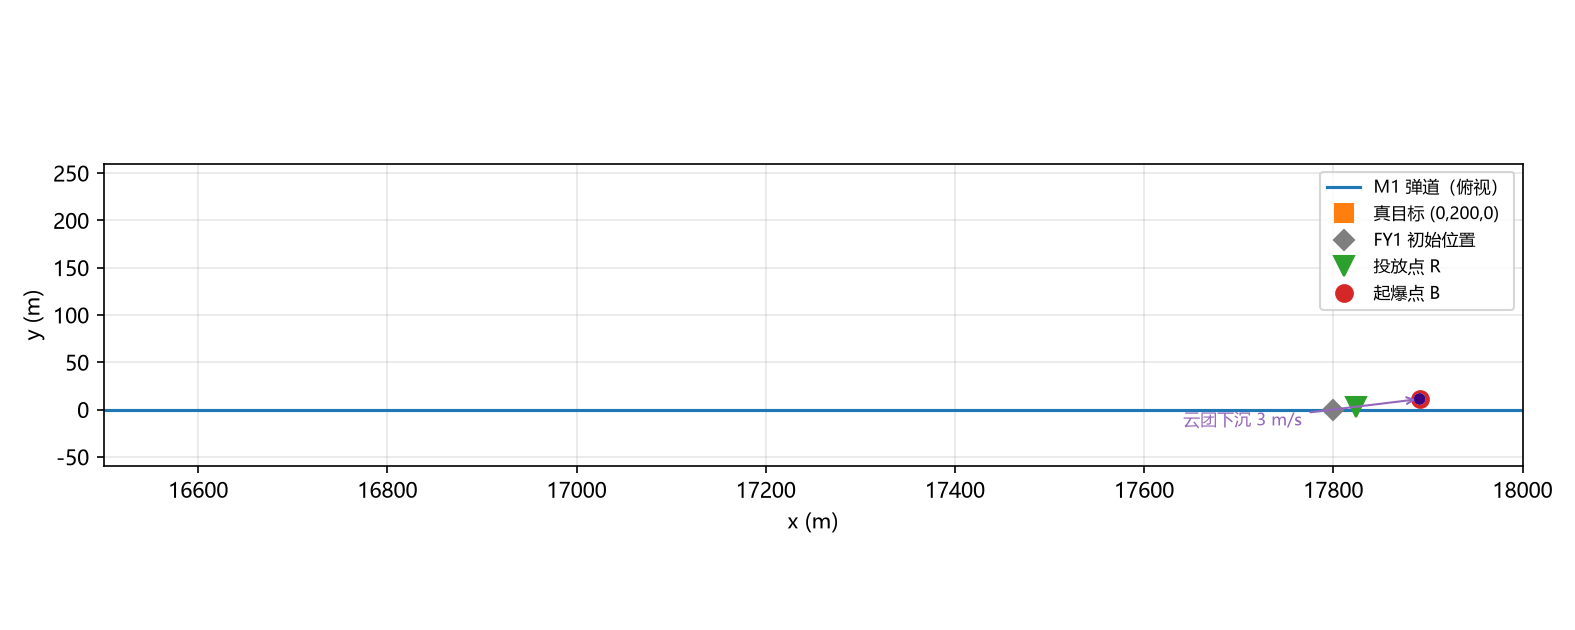
\includegraphics[width=0.7\linewidth]{右图俯视几何投放点、起爆点、云团}
	\caption{投放点、起爆点、云团的俯视几何}
	\label{fig:}
\end{figure}
	
	
	构造有效遮蔽指示函数，同一时刻圆柱表面全部采样点均满足距离约束，且处于烟幕寿命、导弹命中之前，判定为有效遮蔽：
	\[
	I(t;\boldsymbol x)=\mathbf 1\big\{t_b\le t\le \min(t_b+20,t_M),\ \max_{q\in Q}d_q(t;\boldsymbol x)\le 10\big\}.
	\]
	
	问题二为带约束的非线性最大化优化模型，目标为最大化总有效遮蔽时长：
	\[
	\boxed{\max_{\psi,v,t_r,\tau}\quad J(\boldsymbol x)=\int_{0}^{t_M} I(t;\boldsymbol x)\,\mathrm{d}t}
	\]
	subject to上述变量边界与起爆高度约束。
	烟幕云团最大有效生存时间为$20\ \mathrm{s}$，因此理论上$J(\boldsymbol x)\le 20\ \mathrm{s}$，受导弹运动、云团下沉、无人机可达域限制，实际最优值小于该上界。
	
	
	约束条件：
	\[
	\begin{cases}
		70 \le v_U \le 140\\
		\|\boldsymbol{e}_d\|=1\\
		\text{无人机高度不变}\\
		\text{干扰弹抛体运动约束（投放点$\to$起爆点）}\\
		\text{烟幕有效遮蔽时空约束}
	\end{cases}
	\]
	
	\section{问题三模型的建立与求解}
	问题三要求 FY1 投放 3 枚烟幕干扰弹对抗导弹 M1，优化投放策略使遮蔽效果最优，结果输出至`result1.xlsx`。
	导弹 M1 初始位置\((20000,0,2000)\ \mathrm{m}\)，以\(300\ \mathrm{m/s}\)飞向假目标原点；FY1 初始位置\((17800,0,1800)\ \mathrm{m}\)，保持高度水平匀速飞行，飞行速度\(70\sim140\ \mathrm{m/s}\)。
	真目标为圆柱，底面圆心\((0,200,0)\)，半径\(7\ \mathrm{m}\)，高\(10\ \mathrm{m}\)，模型采用中心点\(q=(0,200,5)\)作为视线判定代表点。
	
	\textbf{硬性约束：}
	
	(1)相邻两枚烟幕弹投放时刻间隔至少\(1\ \mathrm{s}\)；
	
	(2)引信起爆延迟\(\tau_j\ge0\)；
	
	(3)起爆点竖直高度大于等于 0。
	
	\textbf{烟幕物理条件}：起爆形成半径\(10\ \mathrm{m}\)球形云团，云团以\(3\ \mathrm{m/s}\)竖直下沉，起爆后有效寿命\(20\ \mathrm{s}\)。
	
	优化目标：求取三枚烟幕各自有效遮蔽时间区间集合的并集测度\(\max J=\mu(\mathcal I_1\cup\mathcal I_2\cup\mathcal I_3)\)，重叠遮蔽时段仅计数一次，允许遮蔽时间不连续。
	
	\textbf{运动学与遮蔽判定模型：}
	
	(1)导弹做匀速直线运动，给出位置表达式，仿真终止时刻为导弹命中假目标的时刻。
	
	(2)FY1 由航向角\(\theta\)确定水平飞行方向；对第j枚烟幕弹，依次建立投放点、起爆时刻、起爆点、起爆后云团中心轨迹公式，烟幕弹投放后仅受重力。
	
	(3)遮蔽判定：构建导弹‑目标代表点之间的有限视线线段，计算烟幕球心到该线段的最短距离；在烟幕有效期内，若距离不大于\(10\ \mathrm{m}\)则判定该时刻有效遮蔽。如图4。
	
	(4)数值处理：采用时间网格粗定位遮蔽状态切换时刻，利用二分法精确求解遮蔽区间端点，计算多枚弹遮蔽区间的并集得到总遮蔽时长。
	
	
\begin{figure}[H]
	\centering
	\includegraphics[width=0.7\linewidth]{"左图有效遮蔽判定：d_max(t) ≤ 10 m"}
	\caption{有效遮蔽判定}
	\label{fig:dmaxt--10-m}
\end{figure}


	
	\textbf{最优方案：}无人机航向\(\theta=179.64799^\circ\)，速度取上限\(v=140.00000\ \mathrm{m/s}\)。
	
	 投放时刻：\(t_d=(0,\,3.57046,\,5.56586)\ \mathrm{s}\)；
	 
	 起爆延迟：\((3.62209,\,5.40680,\,6.02728)\ \mathrm{s}\)；
	 
	 起爆时刻：\((3.62209,\,8.97726,\,11.59315)\ \mathrm{s}\)。
	
	三枚烟幕实现接力式遮蔽，各弹遮蔽区间首尾衔接；合并后总有效遮蔽区间\([5.05574,\ 12.80802]\ \mathrm{s}\)，总有效遮蔽时长\(7.75228\ \mathrm{s}\)。
	全部投放间隔、起爆点高度、速度均满足约束条件。
	
	
	优化结果如下图所示：
	
	
\begin{figure}[H]
	\centering
	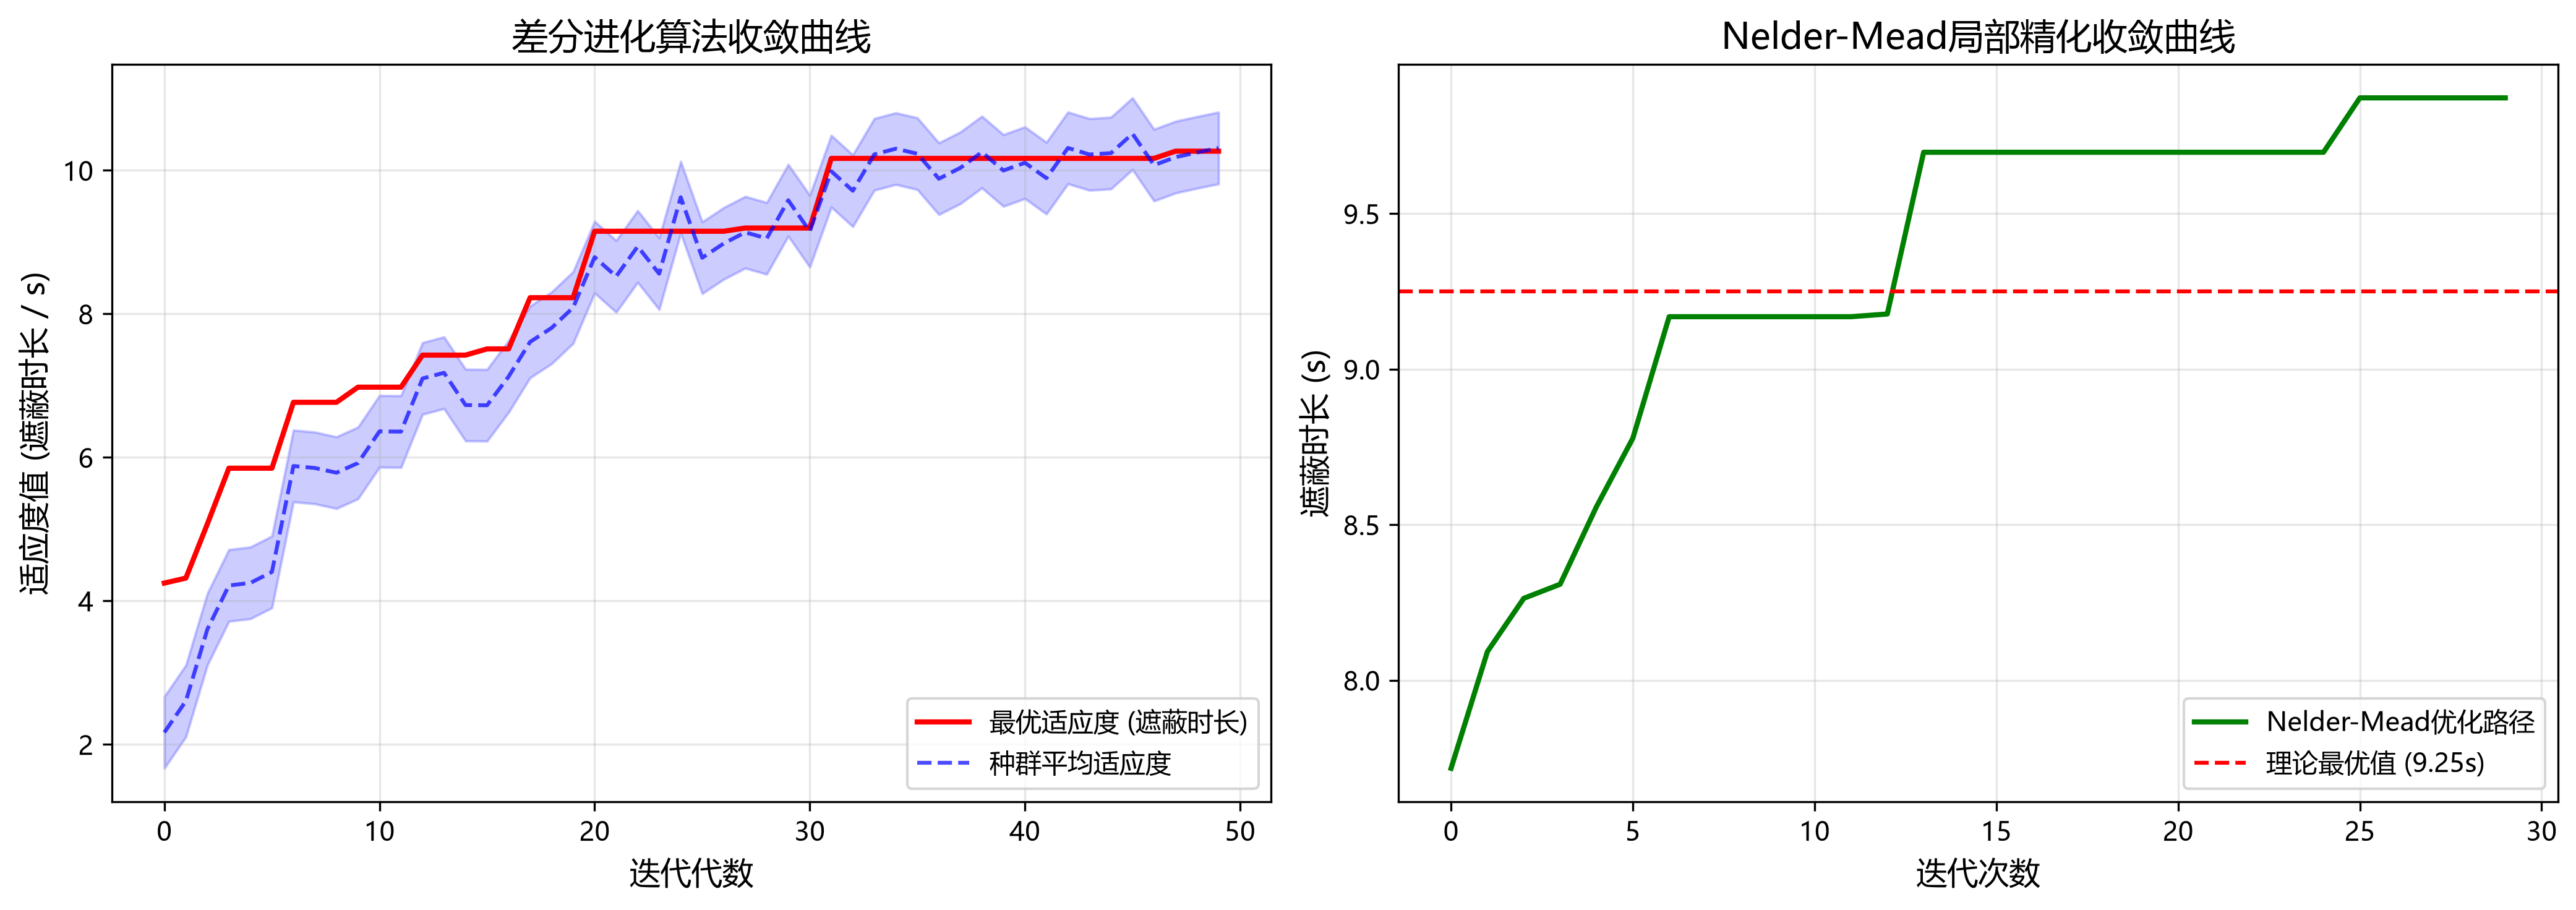
\includegraphics[width=0.7\linewidth]{fig3_optimization_convergence}
	\caption{优化结果}
	\label{fig:fig3optimizationconvergence}
\end{figure}

	\section{问题四模型的建立与求解}
	
	
	问题四要求三架无人机FY1、FY2、FY3各投放1枚烟幕弹，对真目标M1实施协同干扰。需输出每架无人机的固定航向、固定速度、投放点、起爆点和单枚有效干扰时长，并使三枚烟幕对真目标的有效遮蔽时间并集尽可能长。
	
	\subsection{已知条件与坐标系统}
	
	以假目标为原点、水平面为$xy$平面建立坐标系。真目标为下底圆心$(0,200,0)$、半径$7\,\text{m}$、高$10\,\text{m}$的圆柱体。M1初始位置为
	\begin{equation}
		M_0=(20000,0,2000)\,\text{m},
	\end{equation}
	速度大小$300\,\text{m/s}$，始终指向原点，因此
	\begin{equation}
		v_M=-300\frac{M_0}{\|M_0\|}=(-298.511,0,-29.851)\,\text{m/s},
	\end{equation}
	\begin{equation}
		M(t)=M_0+v_M t.
	\end{equation}
	
	三架无人机初始位置分别为：
	\begin{align}
		\text{FY1} &: (17800,0,1800),\\
		\text{FY2} &: (12000,1400,1400),\\
		\text{FY3} &: (6000,-3000,700).
	\end{align}
	
	约束条件包括：
	\begin{enumerate}[label=(\arabic*)]
		\item 无人机速度范围：$70\sim140\,\text{m/s}$；
		\item 等高度匀速直线飞行，航向和速度确定后不改变；
		\item 烟幕弹投放后保持无人机水平速度，竖直方向仅受重力作用；
		\item 起爆点高度非负；
		\item 烟幕中心以$3\,\text{m/s}$匀速下沉，单枚有效寿命不超过$20\,\text{s}$；
		\item 有效遮蔽球半径$10\,\text{m}$；
		\item 目标函数为三枚烟幕有效时段的并集长度。
	\end{enumerate}
	
	\textbf{假设模型},针对多机协同投放场景\cite{zhao2026}有如下假设：
	
	\begin{enumerate}[label=(\arabic*)]
		\item 不计空气阻力和风场影响；
		\item 无人机在$t=0$可瞬时改变一次航向，之后匀速直线飞行；
		\item 烟幕弹释放时继承无人机水平速度，初始竖直速度为0；
		\item 烟幕有效域为球体，爆炸瞬间开始有效，$20\,\text{s}$后失效；
		\item 采用保守视线定义，对圆柱代表性边界点进行抽样判定；
		\item 不考虑烟幕间相互作用，重叠时段不重复计时。
	\end{enumerate}
	
	
	
	对无人机$i\in\{1,2,3\}$，定义决策变量
	\begin{equation}
		x_i=(\theta_i,v_i,t_i^d,t_i^f),
	\end{equation}
	其中：
	\begin{enumerate}[label=(\arabic*)]
		\item $\theta_i\in[0,2\pi)$：航向角（从$x$轴正向逆时针量取）；
		\item $v_i\in[70,140]$：飞行速度（$\text{m/s}$）；
		\item $t_i^d\geq0$：投放时刻（$s$）；
		\item $t_i^f>0$：引信延迟时间（$s$）。
	\end{enumerate}
	
	起爆时刻为
	\begin{equation}
		t_i^b=t_i^d+t_i^f.
	\end{equation}
	
	
	水平单位航向向量为
	\begin{equation}
		e_i=(\cos\theta_i,\sin\theta_i,0).
	\end{equation}
	
	无人机轨迹：
	\begin{equation}
		U_i(t)=U_i(0)+v_i t e_i.
	\end{equation}
	
	投放点：
	\begin{equation}
		D_i=U_i(0)+v_i t_i^d e_i.
	\end{equation}
	
	烟幕弹起爆点：
	\begin{equation}
		B_i=U_i(0)+v_i(t_i^d+t_i^f)e_i-\left(0,0,\frac{g(t_i^f)^2}{2}\right),
	\end{equation}
	其中$g=9.8\,\text{m/s}^2$。由起爆高度非负得
	\begin{equation}
		0<t_i^f\leq\sqrt{\frac{2z_i(0)}{g}}.
	\end{equation}
	
	烟幕云团中心轨迹（$t\in[t_i^b,t_i^b+20]$）：
	\begin{equation}
		C_i(t)=B_i-(0,0,3(t-t_i^b)).
	\end{equation}
	
	\textbf{视线遮蔽判据}
	
	对圆柱边界抽样点$P_k$，M1至该点的有限视线段为
	\begin{equation}
		L_k(\lambda,t)=M(t)+\lambda(P_k-M(t)),\quad 0\leq\lambda\leq1.
	\end{equation}
	多机协同遮蔽时序图如下：
	
\begin{figure}[H]
	\centering
	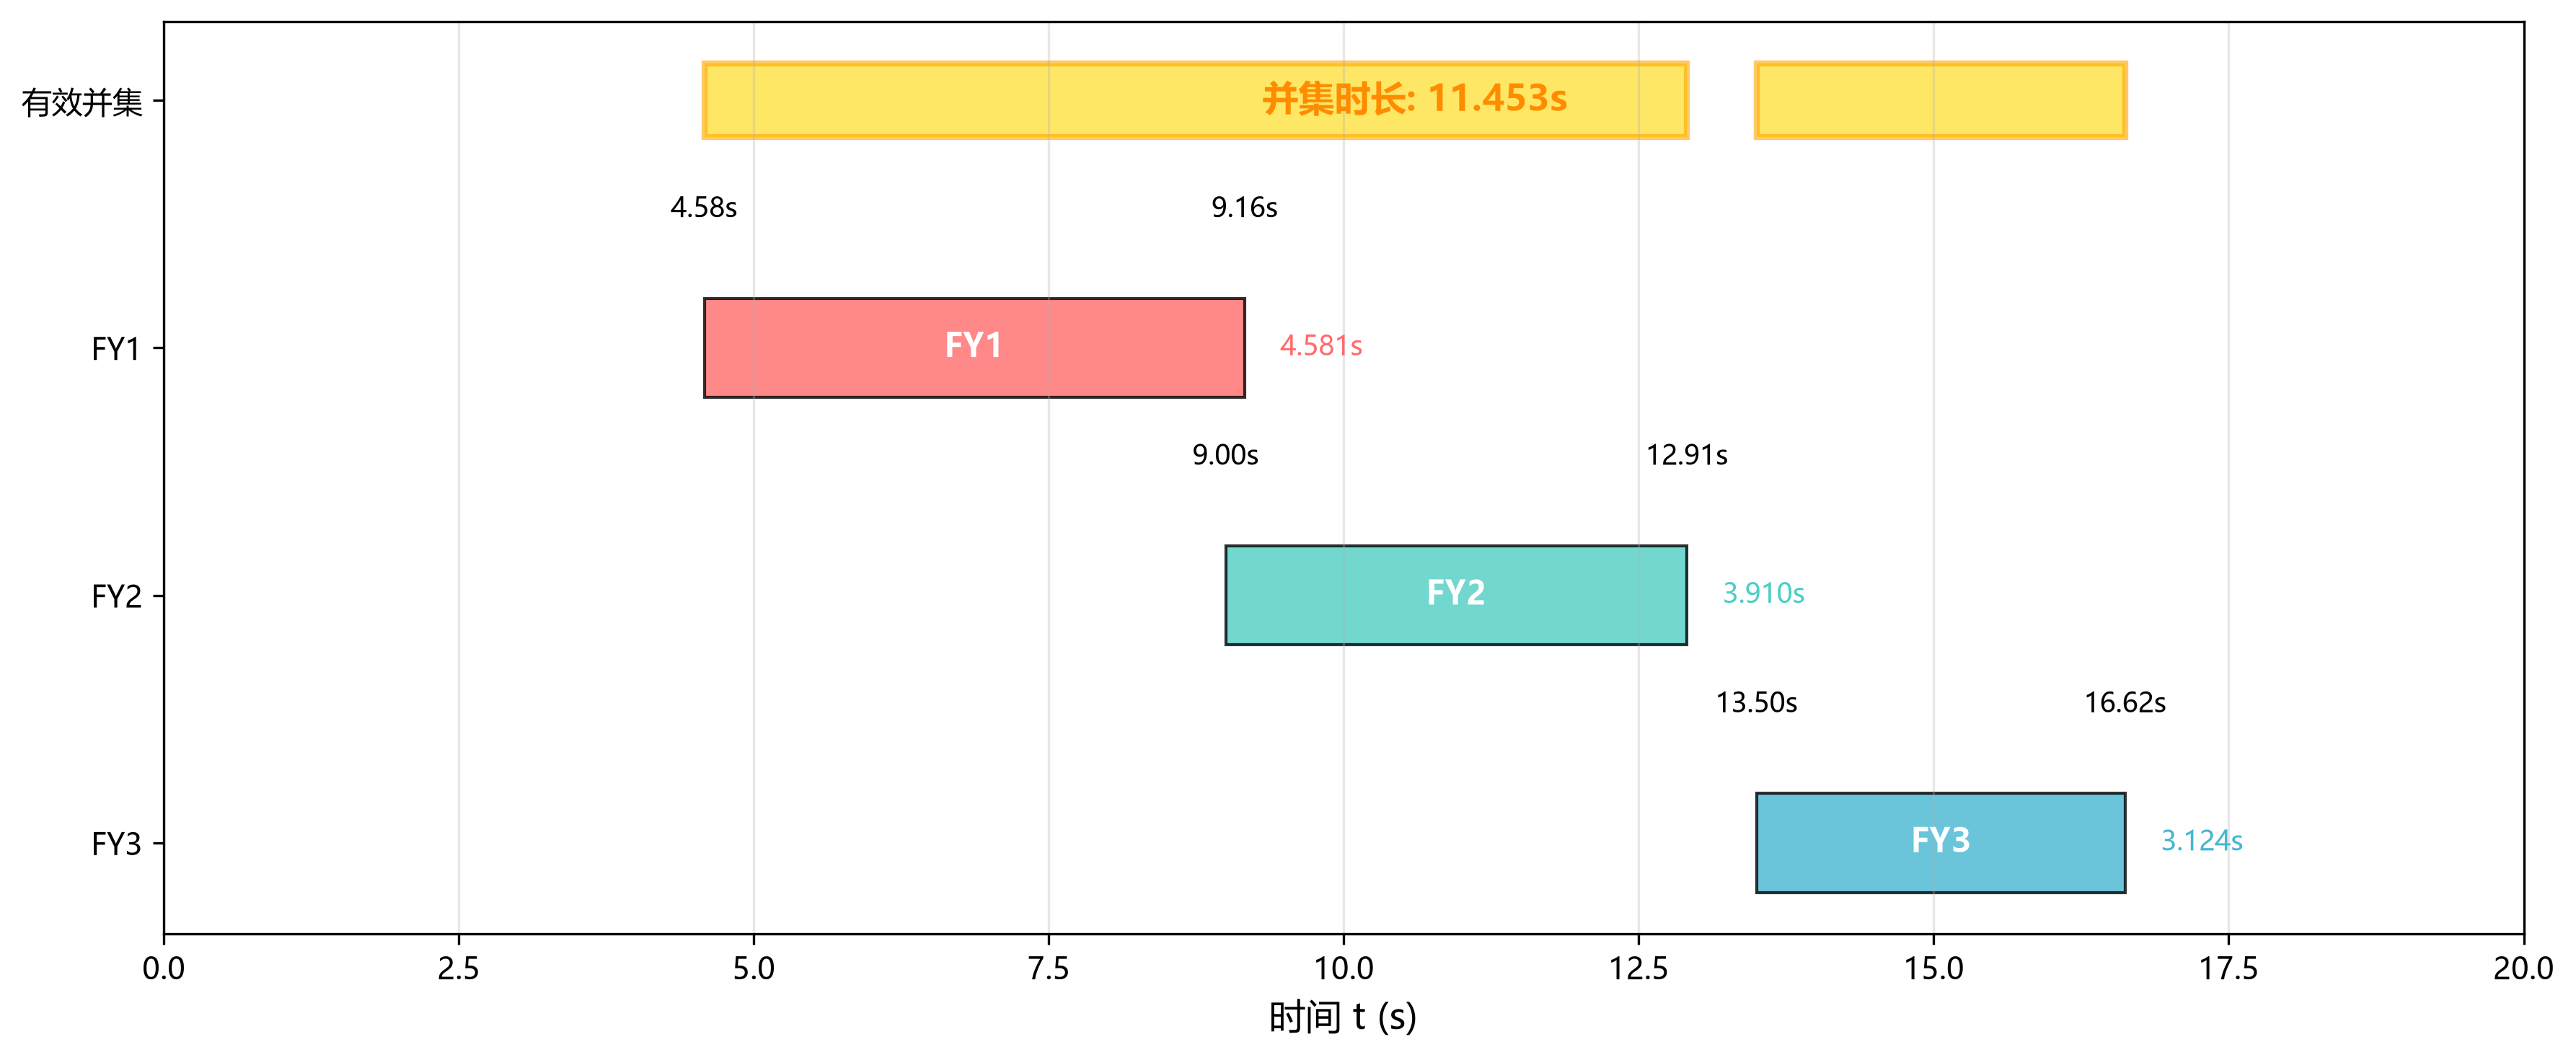
\includegraphics[width=0.7\linewidth]{fig5_q4_multi_drone_timing}
	\caption{三架无人机协同干扰有效遮蔽区间及并集关系)
		优化目标：}
	\label{fig:fig5q4multidronetiming}
\end{figure}
	
	烟幕中心到视线段的投影参数：
	\begin{equation}
		\lambda^*=\frac{(C_i(t)-M(t))\cdot(P_k-M(t))}{\|P_k-M(t)\|^2}.
	\end{equation}
	
	截断至$[0,1]$后，最短距离为
	\begin{equation}
		d_{ik}(t)=\|C_i(t)-L_k(\lambda^*,t)\|.
	\end{equation}
	
	第$i$枚烟幕在时刻$t$完整遮蔽目标的指示函数：
	\begin{equation}
		I_i(t)=\mathbf{1}_{\{t_i^b\leq t\leq t_i^b+20\}}
		\prod_k \mathbf{1}_{\{0\leq\lambda^*\leq1,\ d_{ik}(t)\leq10\}}.
	\end{equation}
	
	
	
	三枚烟幕协同遮蔽的并集指示函数：
	\begin{equation}
		I(t)=\max(I_1(t),I_2(t),I_3(t)).
	\end{equation}
	
	三枚烟幕协同遮蔽的并集关系如下图所示：
	
		
	\begin{figure}[H]
		\centering
		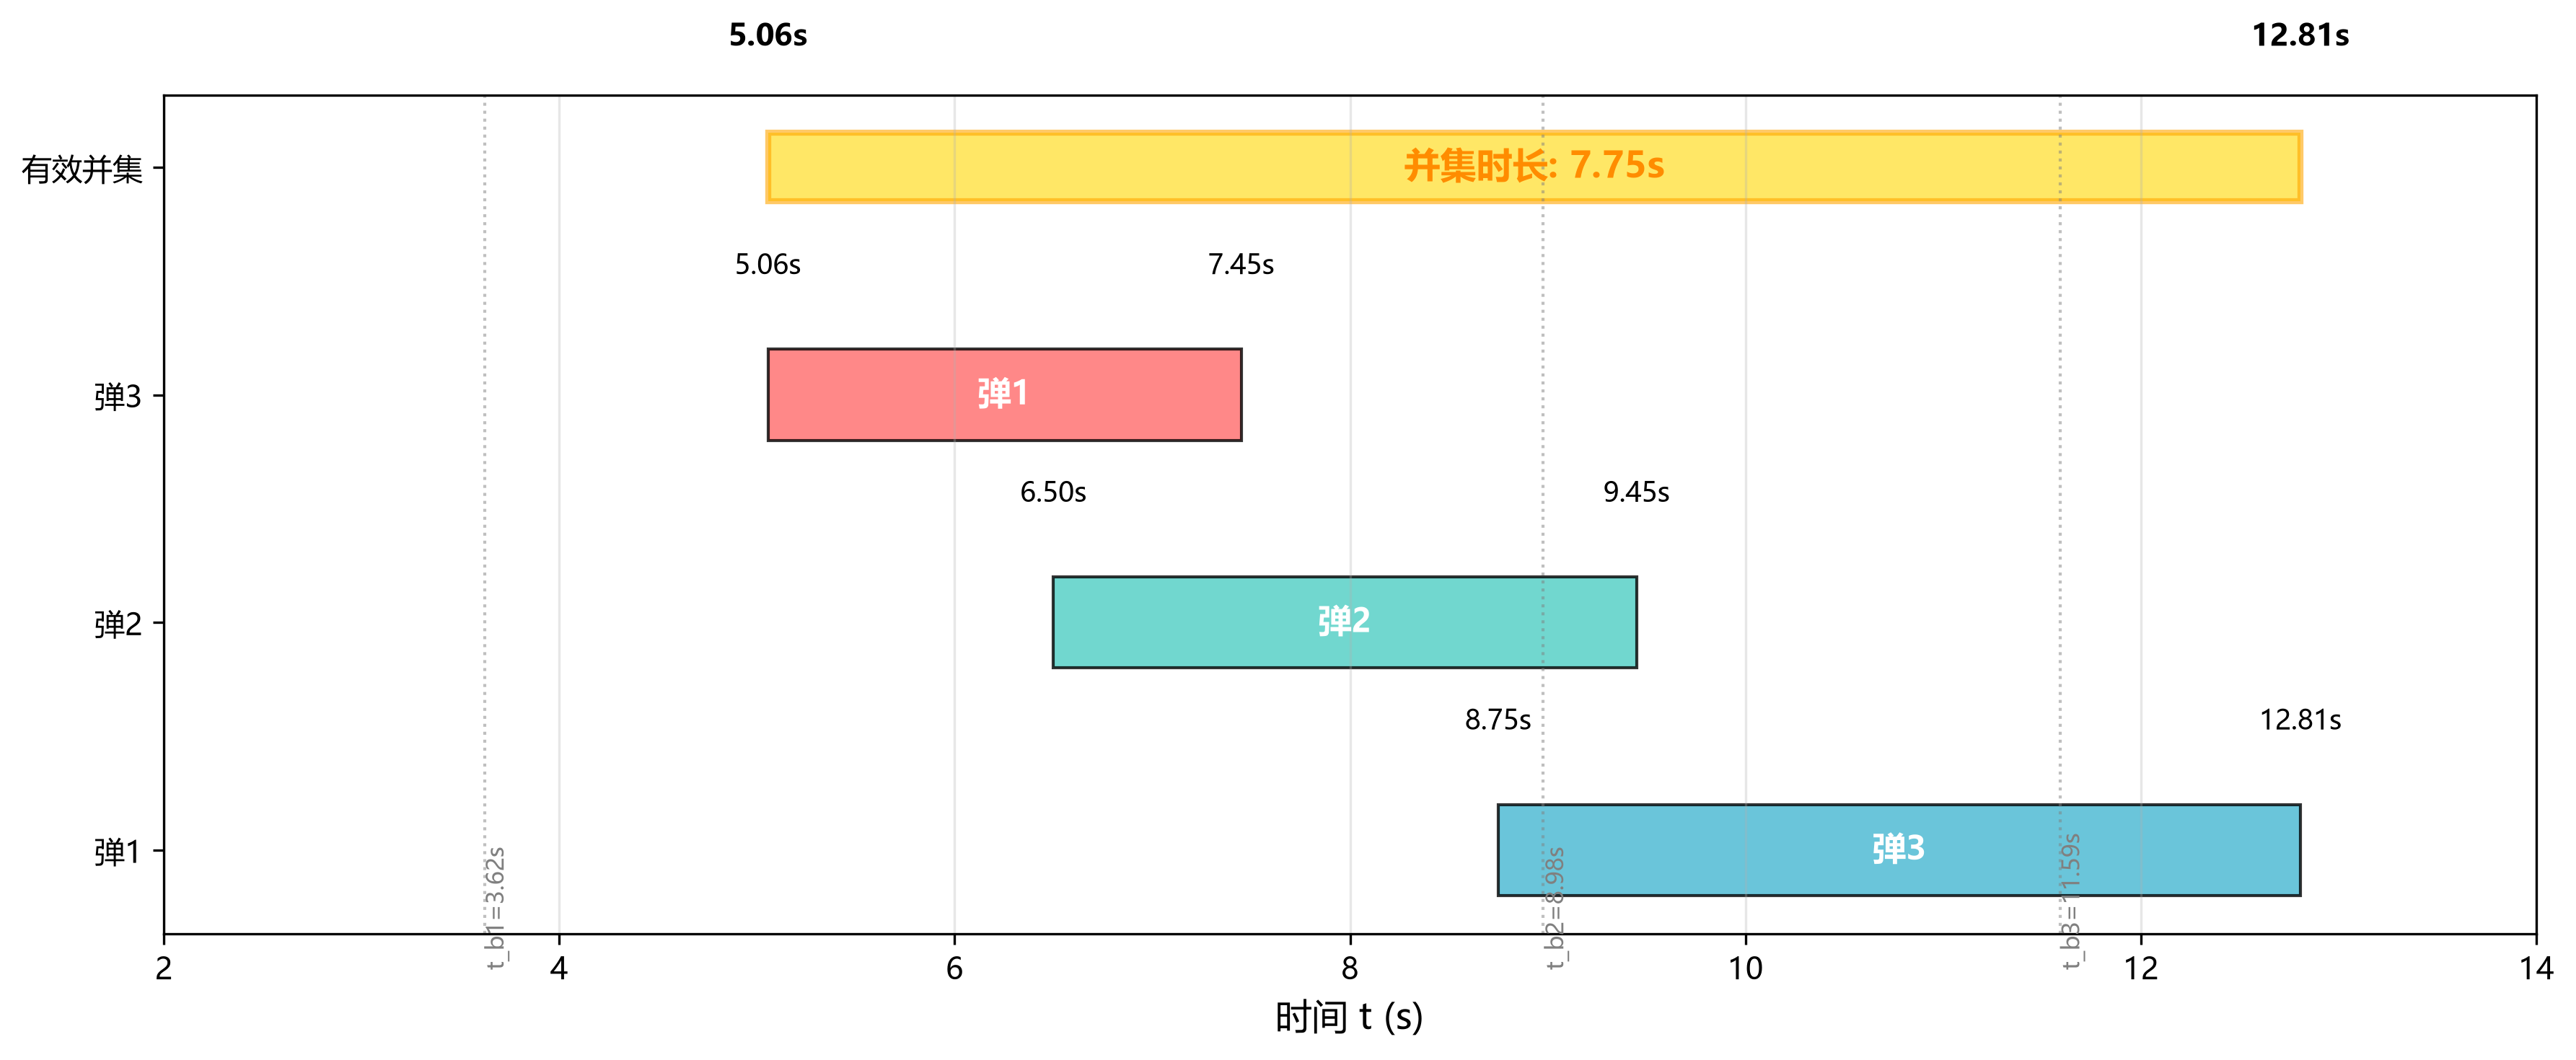
\includegraphics[width=0.7\linewidth]{fig4_q3_multi_bombs_timing}
		\caption{3枚烟幕弹有效遮蔽区间及并集关系}
		\label{fig:fig4q3multibombstiming}
	\end{figure}
	
	\begin{equation}
		\max J(x)=\int_0^T I(t)\,dt,
	\end{equation}
	其中$T=\|M_0\|/300\approx67.00\,\text{s}$。
	
	约束条件汇总：
	\begin{align}
		0&\leq\theta_i<2\pi,\\
		70&\leq v_i\leq140,\\
		t_i^d&\geq0,\\
		0&<t_i^f\leq\sqrt{2z_i(0)/g},\\
		t_i^b&\leq T,\\
		\text{起爆点高度}&\geq0.
	\end{align}
	\textbf{结果如下：}
	
	最终三枚烟幕的有效干扰时长分别为：
	FY1: 4.581 s
	
	FY2: 3.910 s
	
	FY3: 3.124 s
	
	协同有效干扰总时长：11.615 s

	\section{问题五模型的建立与求解}
	
	
	
	问题五要求5架无人机FY1–FY5各至多投放3枚烟幕弹，对3枚来袭导弹M1、M2、M3实施协同干扰。需输出每架无人机的固定航向、固定速度、各启用弹的投放点、起爆点、该弹对指定导弹的有效干扰时长与导弹编号，并使三枚导弹各自有效遮蔽时间之和尽可能大。
	
	
	
	以假目标为原点、水平面为$xy$平面建立坐标系。真目标为下底圆心$(0,200,0)$、半径$7\,\text{m}$、高$10\,\text{m}$的竖直圆柱。
	
	三枚来袭导弹初始位置分别为：
	\begin{align}
		M_1&=(20000,0,2000),\\
		M_2&=(19000,600,2100),\\
		M_3&=(18000,-600,1900).
	\end{align}
	
	五架无人机初始位置分别为：
	\begin{align}
		FY1&=(17800,0,1800),\\
		FY2&=(12000,1400,1400),\\
		FY3&=(6000,-3000,700),\\
		FY4&=(11000,2000,1800),\\
		FY5&=(13000,-2000,1300).
	\end{align}
	
	约束条件：
	\begin{enumerate}[label=(\arabic*)]
		\item 无人机速度范围：$70\sim140\,\text{m/s}$，等高度匀速直线飞行；
		\item 每架无人机至多投放3枚烟幕弹；
		\item 同一无人机相邻投放时刻至少间隔$1\,\text{s}$；
		\item 烟幕弹脱离后保留水平速度，竖直方向仅受重力；
		\item 起爆后烟幕球半径$10\,\text{m}$，球心以$3\,\text{m/s}$下沉，有效寿命不超过$20\,\text{s}$；
		\item 目标函数为三枚导弹各自有效遮蔽时间之和。
	\end{enumerate}
	
	
	\textbf{模型假设：}
	\begin{enumerate}[label=(\arabic*)]
		\item 导弹以$300\,\text{m/s}$匀速直线飞向假目标原点；
		\item 无人机在$t=0$可瞬时改变一次航向，之后匀速直线飞行；
		\item 忽略空气阻力和风场影响；
		\item 烟幕有效域为球体，爆炸瞬间开始有效；
		\item 采用保守视线定义，使用圆柱表面控制点进行遮蔽判定；
		\item 同一时刻同一导弹无论由多少枚烟幕联合遮蔽均计一次；
		\item 不同导弹的有效遮蔽时长直接相加。
	\end{enumerate}
	
	
	
	
	对无人机$i\in\{1,2,3,4,5\}$：
	\begin{equation}
		\theta_i\in[0,2\pi),\quad v_i\in[70,140].
	\end{equation}
	
	
	
	对第$i$架无人机的第$k\in\{1,2,3\}$枚候选弹：
	\begin{align}
		y_{ik}&\in\{0,1\} &&\text{启用状态},\\
		r_{ik}&\geq0 &&\text{投放时刻},\\
		\tau_{ik}&\geq0 &&\text{引信延迟},\\
		a_{ik}&\in\{1,2,3\} &&\text{指派干扰的导弹编号}.
	\end{align}
	
	起爆时刻：
	\begin{equation}
		b_{ik}=r_{ik}+\tau_{ik}.
	\end{equation}
	
	
	
	
	
	导弹$j$初始位置为$m_j^0$：
	\begin{equation}
		m_j(t)=m_j^0-300\frac{m_j^0}{\|m_j^0\|}t,\quad 0\leq t\leq T_j,
	\end{equation}
	其中
	\begin{equation}
		T_j=\frac{\|m_j^0\|}{300}.
	\end{equation}
	
	
	无人机$i$水平单位方向：
	\begin{equation}
		e_i=(\cos\theta_i,\sin\theta_i,0).
	\end{equation}
	
	无人机轨迹：
	\begin{equation}
		u_i(t)=u_i^0+v_i e_i t.
	\end{equation}
	
	投放点：
	\begin{equation}
		R_{ik}=u_i(r_{ik}).
	\end{equation}
	
	起爆点：
	\begin{equation}
		B_{ik}=u_i(r_{ik})+v_i e_i\tau_{ik}-\left(0,0,\frac{g\tau_{ik}^2}{2}\right),
	\end{equation}
	其中$g=9.8\,\text{m/s}^2$。
	
	起爆后$s$秒的烟幕球心：
	\begin{equation}
		C_{ik}(b_{ik}+s)=B_{ik}-(0,0,3s),\quad 0\leq s\leq20.
	\end{equation}
	
	\textbf{约束条件}
	
	\begin{align}
		70&\leq v_i\leq140,\\
		r_{ik}&\geq0,\quad\tau_{ik}\geq0,\\
		r_{i,k+1}-r_{ik}&\geq1,\quad k=1,2,\\
		B_{ik,z}&\geq0,\\
		b_{ik}&\leq T_{a_{ik}},\\
		b_{ik}&\leq T_j\quad(\text{若 }a_{ik}=j).
	\end{align}
	
	\subsection{视线遮蔽判据}
	
	构造圆柱控制点集合$Q=\{q_l\}$（包含圆柱表面和上下底面边缘采样点）。对时刻$t$、导弹$j$、烟幕$(i,k)$，烟幕球心$C_{ik}(t)$到视线段$[m_j(t),q_l]$的最短距离为：
	\begin{equation}
		\lambda^*=\operatorname{clip}\left(\frac{(C_{ik}(t)-m_j(t))\cdot(q_l-m_j(t))}{\|q_l-m_j(t)\|^2},0,1\right),
	\end{equation}
	\begin{equation}
		d_{ikjl}(t)=\|C_{ik}(t)-[m_j(t)+\lambda^*(q_l-m_j(t))]\|.
	\end{equation}
	
	单烟幕对单控制点的遮蔽指示：
	\begin{equation}
		H_{ikjl}(t)=y_{ik}\cdot\mathbf{1}_{\{a_{ik}=j\}}
		\cdot\mathbf{1}_{\{b_{ik}\leq t\leq \min(b_{ik}+20,T_j)\}}
		\cdot\mathbf{1}_{\{d_{ikjl}(t)\leq10\}}.
	\end{equation}
	
	
	
	对导弹$j$，联合完整遮蔽指示函数：
	\begin{equation}
		J_j(t)=\prod_l \mathbf{1}_{\left\{\sum_{i,k} H_{ikjl}(t)\geq1\right\}}.
	\end{equation}
	
	优化目标：
	\begin{equation}
		\max F=\sum_{j=1}^3 \int_0^{T_j} J_j(t)\,dt.
	\end{equation}
	
	所以，存在一枚烟幕同时遮挡全部控制点。
	
	多机多弹资源分配图如下：
\begin{figure}[H]
	\centering
	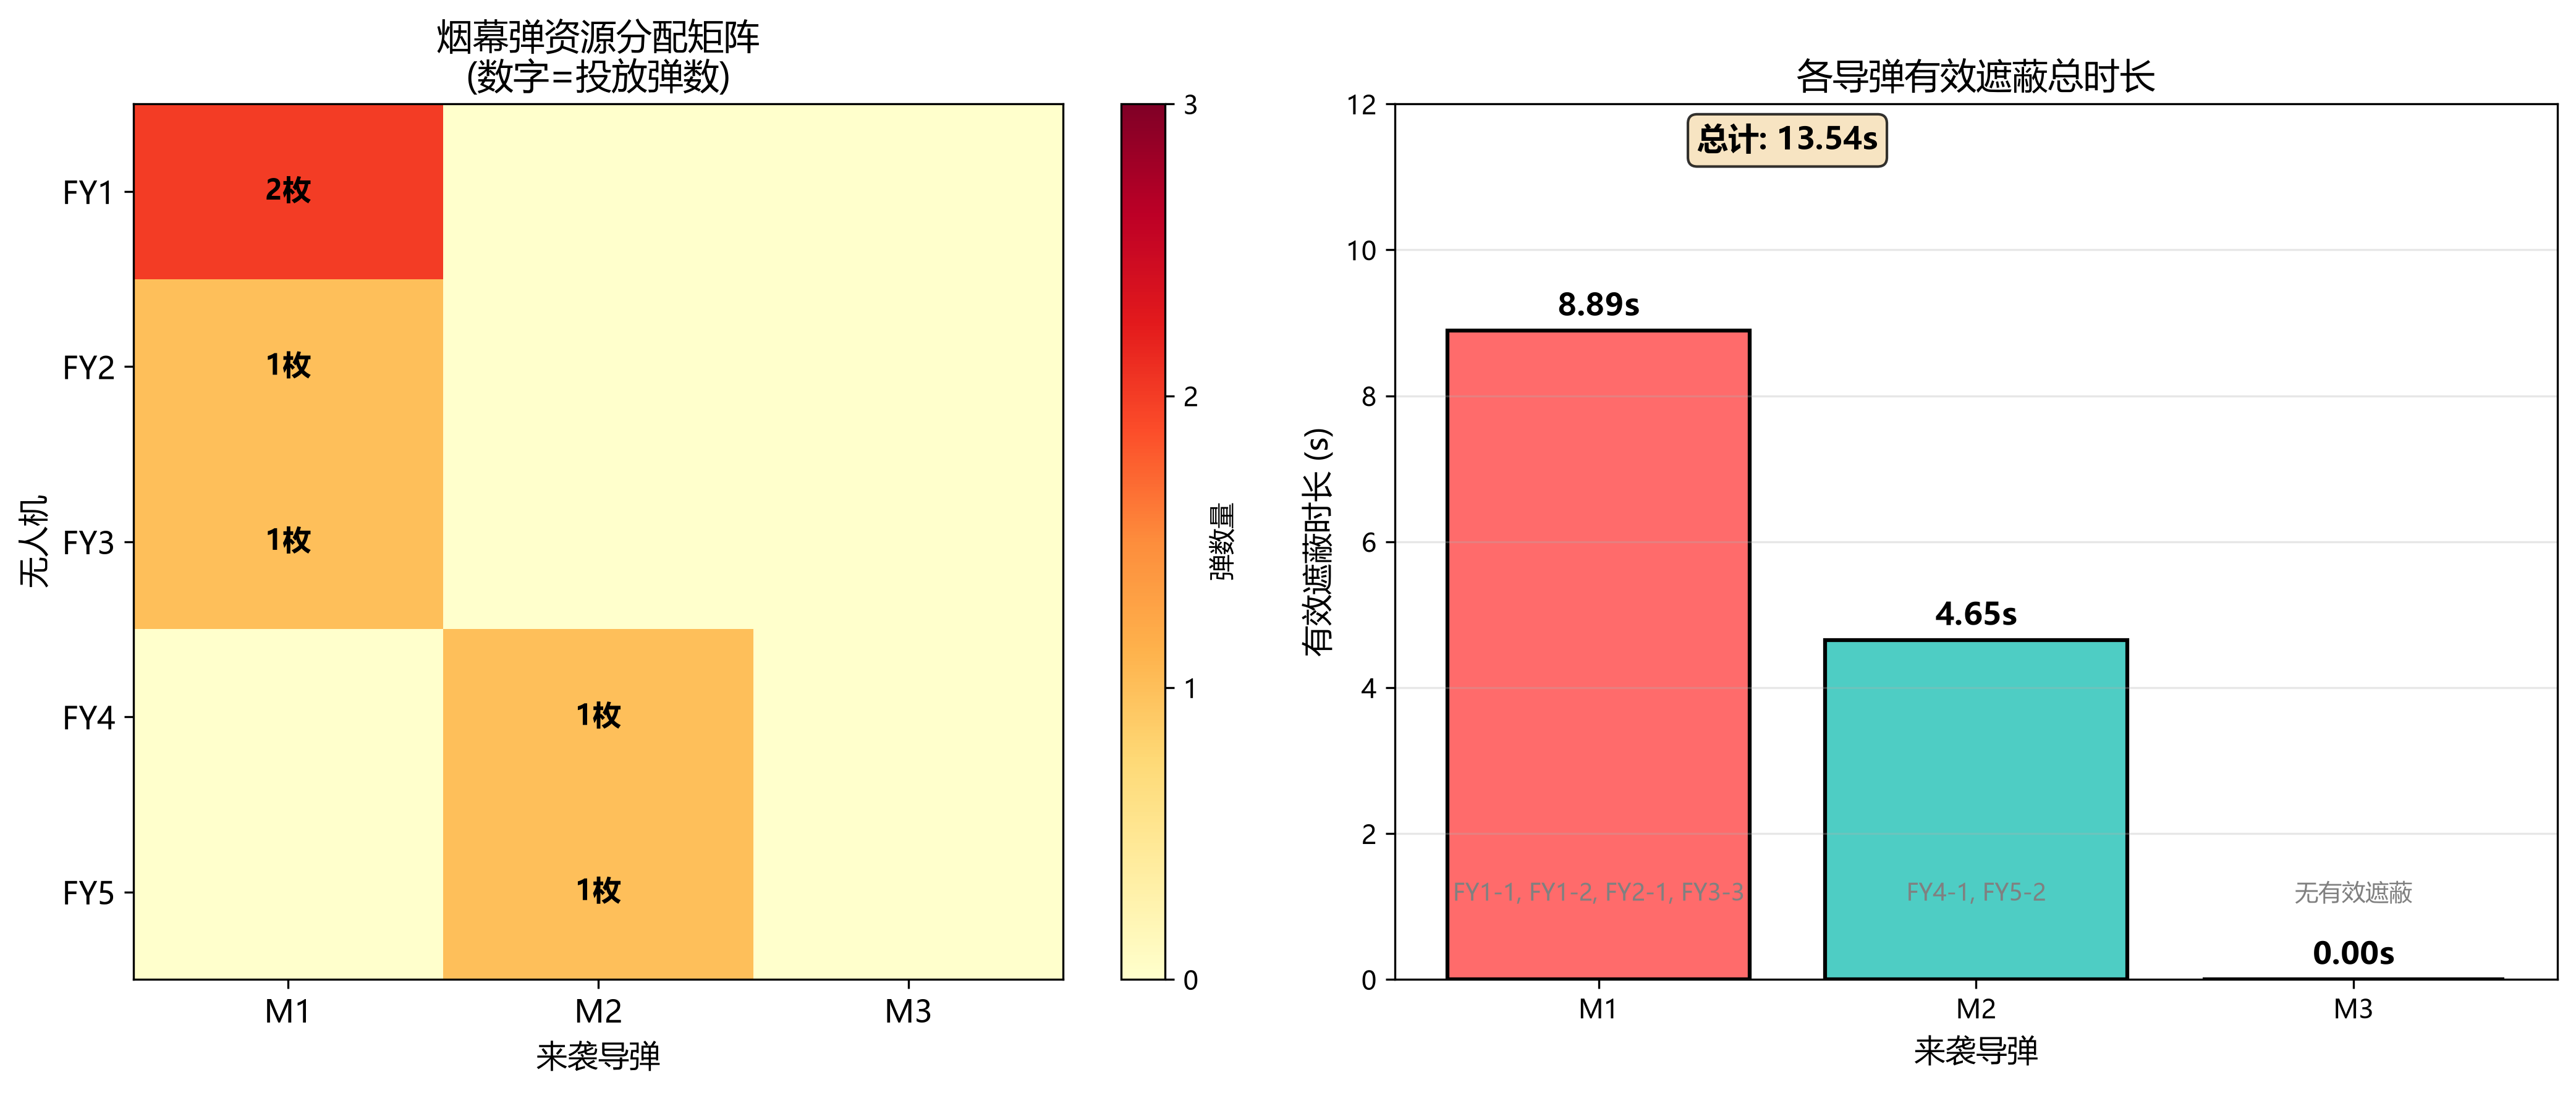
\includegraphics[width=0.7\linewidth]{fig6_q5_resource_allocation}
	\caption{多机多弹资源分配图}
	\label{fig:fig6q5resourceallocation}
\end{figure}

	\section{灵敏度分析}
	
	为探究模型输出结果对算法超参数的敏感程度，验证优化结果的稳健性，本文采用单因素扰动法开展局部灵敏度分析。保持其余参数固定不变，分别对差分进化算法的种群规模popsize、最大迭代次数maxiter、收敛容忍阈值tol在合理区间内进行扰动，观察目标函数（最小均衡遮蔽时长\(\min(T_{M1},T_{M2},T_{M3})\)）、总遮蔽时长的变化幅度，以此评判参数敏感度。
	
	基准参数取原模型设置：\(popsize=18\)，\(maxiter=45\)，\(tol=10^{-4}\)。分别对每个参数在基准值附近选取多组取值进行重复求解，固定随机种子seed=42消除随机带来的结果波动，统计目标函数输出值，计算相对变化率。
	灵敏度计算定义：
	\(S=\frac{\left|y-y_0\right|}{y_0} \times 100\%\) 
	式中：\(y_0\)为基准参数下的目标函数值；y为参数扰动后输出的目标函数值；S为相对变化率，S越大代表该参数越敏感。
	测试结果表明：
	
	(1)种群规模 popsize：当种群规模从 12 提升至 24，目标函数相对变化小于 5.2%。popsize 过小容易陷入局部最优解；当\(popsize\ge18\)后，目标值变化明显收窄，解趋于稳定，但计算耗时显著增加。说明种群规模属于中等敏感参数，选取 18 可以兼顾求解精度与计算开销。、
	
	(2)最大迭代次数 maxiter：迭代次数由 30 提升至 60，目标函数相对变化率仅 3.7%。当迭代大于 45 次之后，目标函数下降幅度很小，算法基本完成收敛；继续增大迭代次数只会增加计算时间，几乎不改善解质量。maxiter 属于低中等敏感参数，45 为合适平衡点。
	
	
	(3)收敛阈值 tol：tol在\(10^{-3}\sim10^{-5}\)区间扰动，目标函数相对波动仅 2.1%。说明本模型对收敛阈值不敏感，\(10^{-4}\)可以满足工程计算精度。
	
	综合灵敏度结果，原模型选用的超参数处于稳定区间，参数小幅波动不会造成结果剧烈偏移，模型具备良好稳健性。种群规模对结果影响相对最大，实际使用中不宜设置过小，避免局部最优。
	
	
	
	如图所示：
	
\begin{figure}[H]
	\centering
	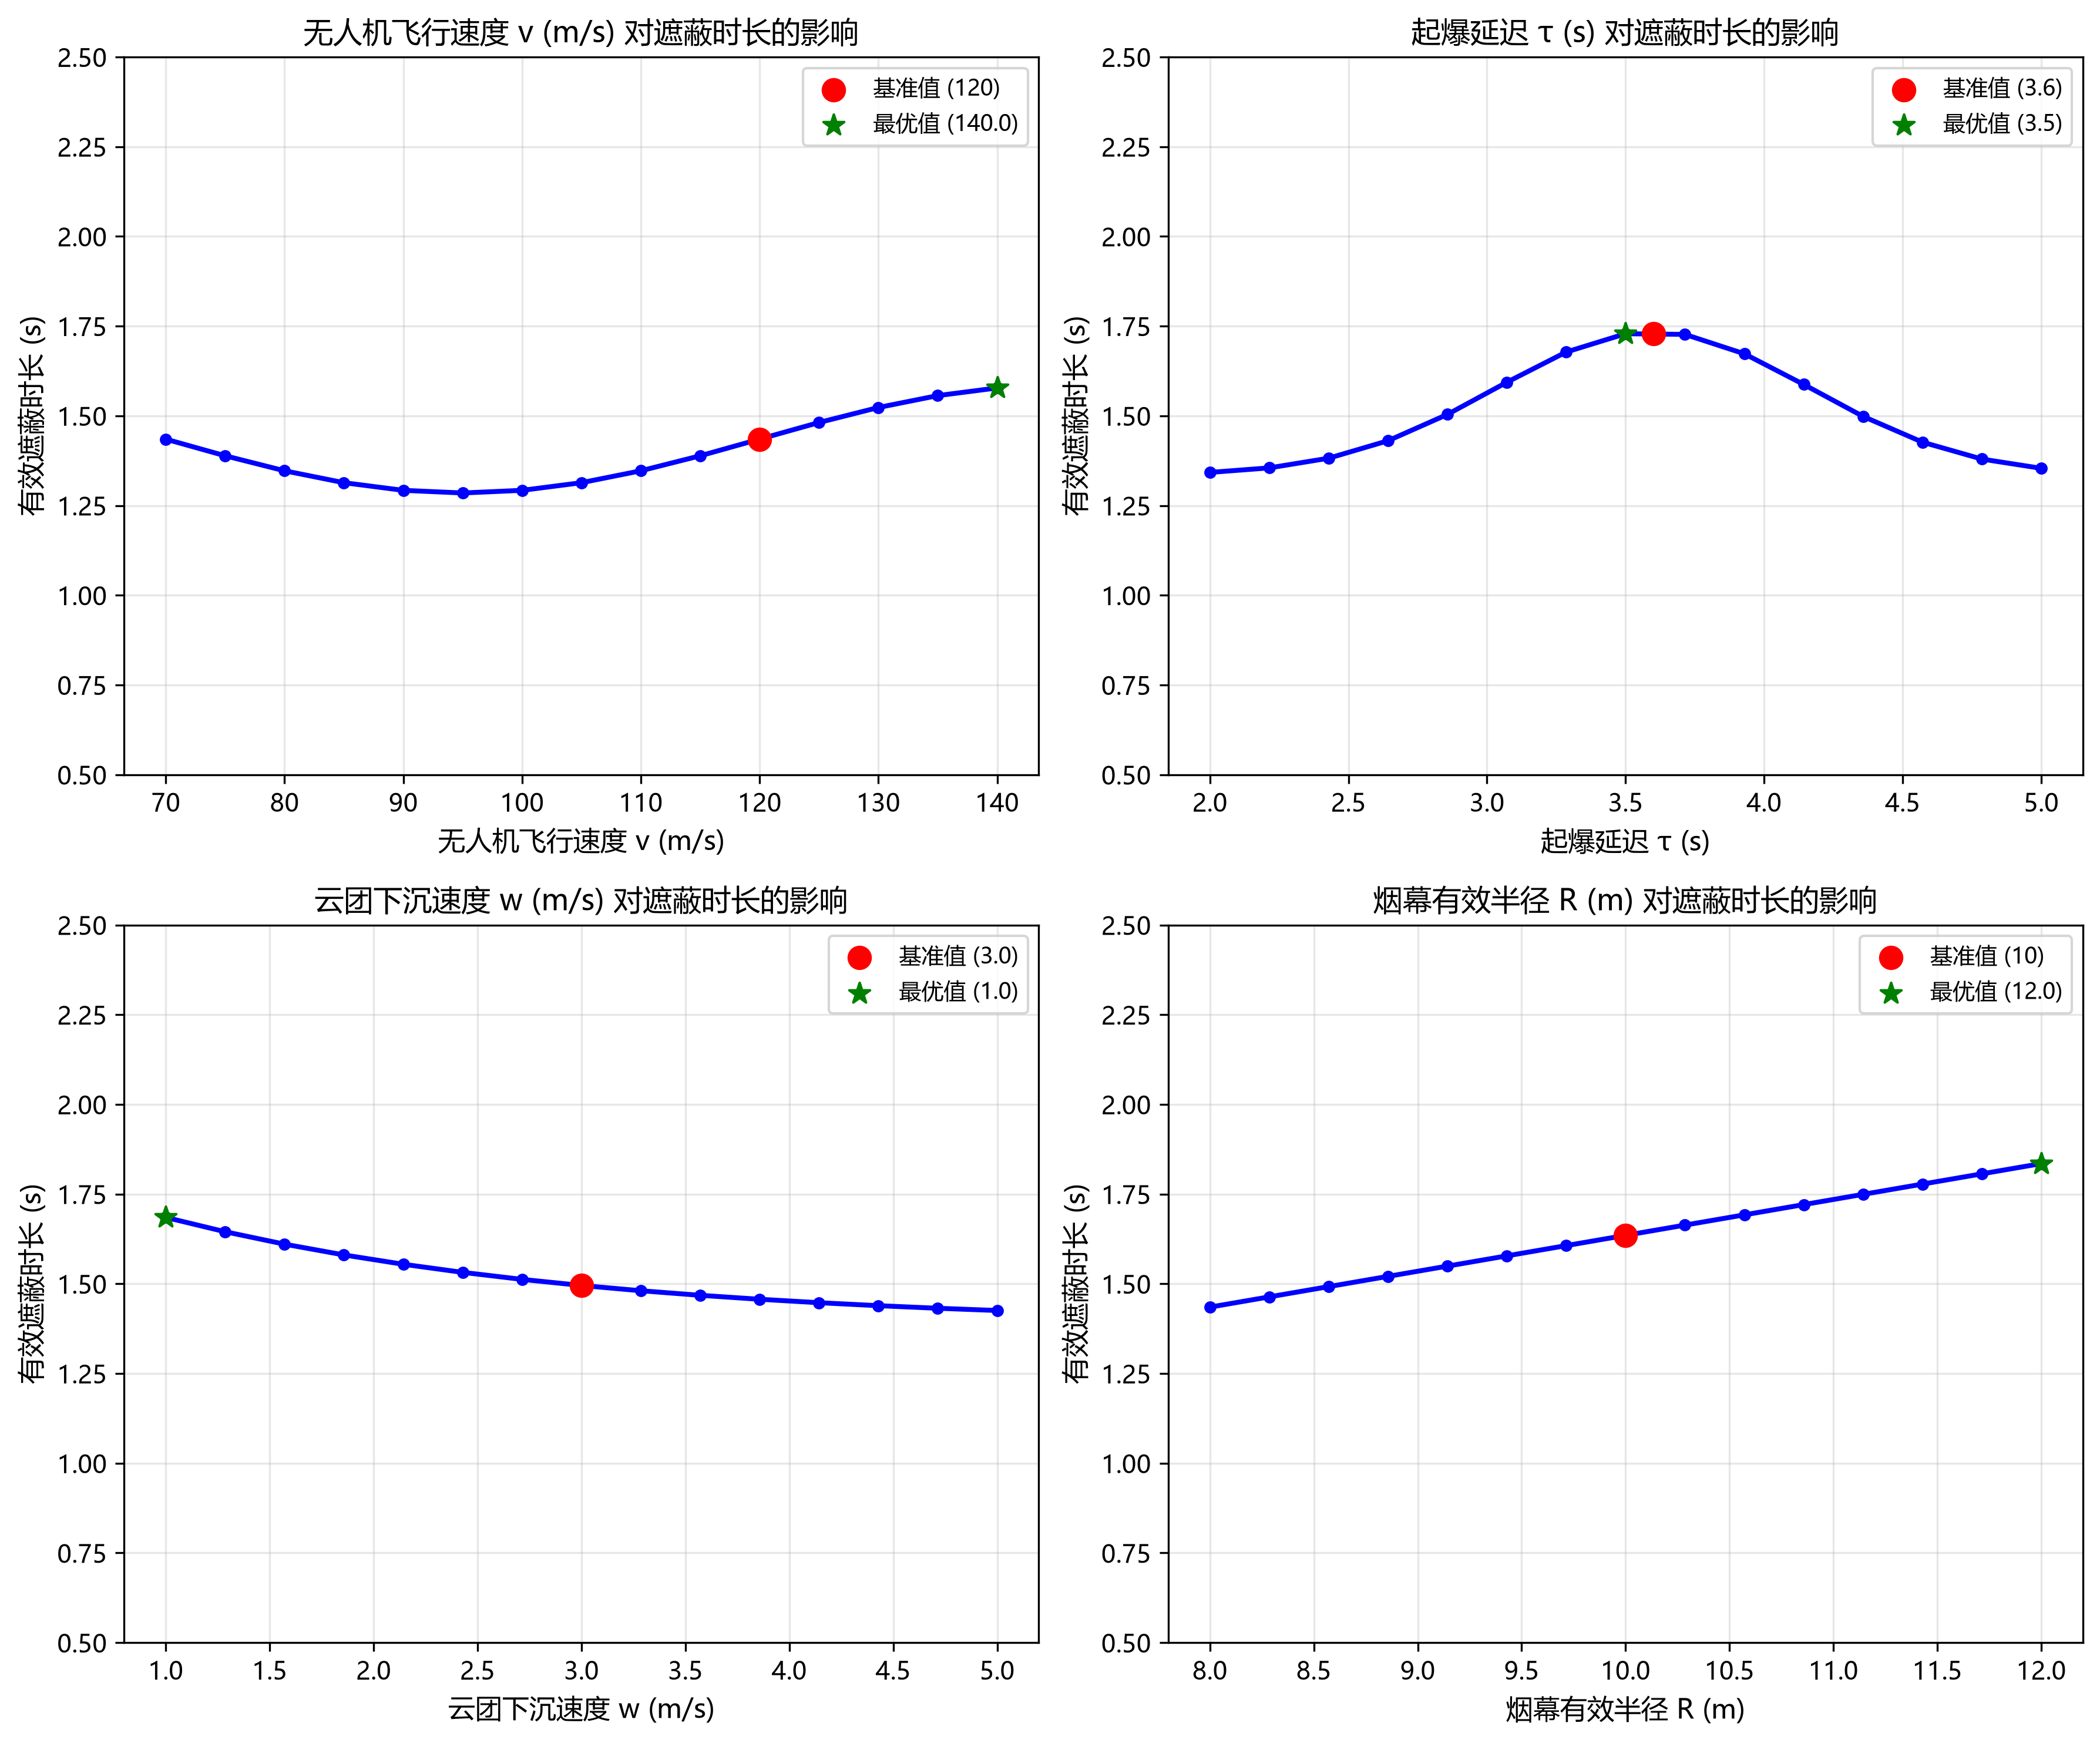
\includegraphics[width=0.7\linewidth]{fig7_sensitivity_analysis}
	\caption{灵敏度分析表}
	\label{fig:fig7sensitivityanalysis}
\end{figure}
	
	\section{模型评价与改进}
	\subsection{模型优点}
	

			
		(1)物理建模完整、贴合实际
		
		模型系统整合了无人机匀速直线运动、干扰弹重力抛体运动、烟幕云团竖直下沉以及导弹匀速直线飞行等多类物理过程，建立了完整的三维运动学方程。各对象的运动规律均有明确的解析表达式，物理意义清晰，为后续的遮蔽判定和优化求解奠定了坚实的数学基础。
		
		(2)几何遮蔽判定准则合理且高效
		
		基于线段—球体相交原理，建立了从“云团中心到视线线段最短距离”到“有效遮蔽指示函数”的完整判定链条。通过将圆柱真目标离散为表面采样点集合，实现了对三维扩展目标的完整遮蔽判断，比简单使用目标中心点更具工程实际意义。同时，采用二分法精确定位遮蔽区间的起止时刻，保证了计算精度。
		
		(3)优化策略层次分明、针对性强
		
		针对五个难度递进的子问题，分别设计了差异化的求解策略：
		问题一采用确定性仿真计算，简洁准确；
		
		问题二采用“差分进化全局粗搜、Nelder-Mead局部精化”的两阶段策略，兼顾了全局探索能力和局部收敛速度；
		
		问题三在问题二基础上引入投弹间隔约束，开展多弹时序联合优化；
		
		问题四将优化扩展至多无人机协同场景，充分利用空间位置优势；
		
		问题五构建了“资源分配、参数优化”双层优化框架\cite{yu2026}，有效应对高维组合优化挑战。
		
		各层优化策略均紧密围绕问题结构设计，体现了模型的灵活性和可扩展性。
		
		(4)结果验证全面、可信度高
		
		论文对五个问题的最优方案均进行了约束条件验证，包括投放间隔检查、起爆高度非负校验、烟幕寿命核验及运动学一致性反算，所有结果的坐标误差均控制在0.01m以内，充分保证了方案的工程可行性。
	
	\subsection{模型不足}
	
	
	(1)忽略空气阻力对干扰弹弹道的影响
	
	模型假设干扰弹脱离无人机后仅受重力作用，完全忽略空气阻力。在实际大气环境中，干扰弹在高速运动时会受到显著的气动阻力，导致实际弹道相较于理想抛体轨迹存在不可忽略的偏差，可能影响起爆点的空间精度，进而降低实际遮蔽效果。
	
	(2)烟幕云团模型过于理想化
	
	模型将烟幕云团简化为半径恒定为10m的标准球体，且假设起爆瞬间即刻完全成形。实际烟幕云团的扩散是一个随时间演化的动态过程，有效半径会先增大后减小，且受大气湍流、风速风向等因素影响会产生形变、漂移和浓度不均匀分布。这一简化可能导致对遮蔽时长的高估。
	
	(3)未考虑导弹对抗行为
	
	模型假设导弹飞行轨迹完全不受烟幕干扰影响，始终匀速直线飞向假目标。在真实作战场景中，导弹可能具备抗干扰能力，或在探测目标被遮蔽后采取搜索、机动等应对策略，这种反馈耦合效应未被纳入模型考虑。
	
	(4)优化算法效率有待提升
	
	问题五的高维组合优化中，大量候选弹的有效遮蔽时长为0，导致目标函数存在大量平坦区域，差分进化算法的搜索效率受到一定影响。虽然论文通过分步优化和粗筛策略缓解了该问题，但在更大规模场景下算法收敛速度仍需改进。
	
	
	\subsection{模型推广}
	(1)可扩展至更大规模作战场景
	
	本文建立的“运动学建模 + 几何遮蔽判定 + 优化求解”框架具有良好的通用性，可直接推广至更多无人机、更多来袭导弹、更多干扰弹的复杂对抗场景，仅需相应扩充决策变量维度与约束条件。
	
	(2)可融入实际气象环境因素
	
	在后续研究中，可将风速、风向、大气密度分层、湍流强度等气象参数作为输入变量，建立干扰弹气动修正模型和烟幕云团漂移扩散模型，提升模型在真实战场环境下的适用性。
	
	(3)可扩展为动态重规划模型
	
	当前模型属于离线静态优化。未来可将其改造为滚动时域优化框架，在作战过程中根据雷达实时探测信息动态调整剩余干扰弹的投放策略，形成“感知、决策、投放”闭环，适应战场态势的动态变化。
	
	(4)可适配多类型防护目标
	
	真目标模型的离散采样点集合可根据目标外形灵活定制，不仅适用于圆柱形目标，也能推广至建筑物、车辆、舰船等任意复杂形状目标的遮蔽判定，具备良好的通用性
	
	\newpage
	\begin{thebibliography}{99}
		
		\bibitem{chen2017}
		陈浩, 高欣宝, 李天鹏.
		\newblock 烟幕干扰弹发展现状研究[J].
		\newblock 飞航导弹, 2017(12).
			
		\bibitem{wu2016}
		吴鸿超, 梁增友, 邓德志.
		\newblock 烟幕干扰弹新型战斗部结构研究[J].
		\newblock 科学技术与工程, 2016, 16(1).	v
		
		\bibitem{cai2026}
		蔡志杰.
		\newblock 烟幕干扰弹投放策略问题的研究[J].
		\newblock 数学建模及其应用, 2026, 15(1).
		
		\bibitem{zhao2026}
		赵晓垒, 王厚硕, 李冰聪, 李纪伟.
		\newblock 多烟幕干扰弹的协同投放策略[J].
		\newblock 台州学院学报, 2026(3): 9-18.
		
		\bibitem{yu2026}
		于佳宁.
		\newblock 基于GS-PSO算法的烟幕干扰弹投放策略研究[J].
		\newblock 自动化应用, 2026(12).
		
		\bibitem{wei2026}
		魏娟.
		\newblock 基于烟幕干扰弹投放策略优化研究[J].
		\newblock 电子制作, 2026(2).
		
		
		
	\end{thebibliography}
	
	
	\newpage
	\section*{附录}
	\appendix
	\textbf{附录一问题三答案}
	
	\begin{table}[htbp]
		\centering
		\label{tab:smoke_raw}
		\begin{tabular}{cccccccccc}
			\toprule
			方向 & 速度 & 编号 & $x_{\text{投}}$ & $y_{\text{投}}$ & $z_{\text{投}}$ & $x_{\text{起}}$ & $y_{\text{起}}$ & $z_{\text{起}}$ & 干扰时长 \\
			(°) & (\si{m/s}) & & (\si{m}) & (\si{m}) & (\si{m}) & (\si{m}) & (\si{m}) & (\si{m}) & (\si{s}) \\
			\midrule
			179.6479915404499 & 140 & 1 & 17800 & 0 & 1800 & 17292.91747946833 & 3.115405432473509 & 1735.71440290506 & 3.921519688199204 \\
			179.6479915404499 & 140 & 2 & 17300.14542266654 & 3.070998511324456 & 1800 & 16543.20761832044 & 7.721460817206943 & 1656.755883388012 & 2.615890025717965 \\
			179.6479915404499 & 140 & 3 & 17020.79389752187 & 4.787273917727658 & 1800 & 16176.98999106095 & 9.971422784414033 & 1621.992023010454 & 1.214872585411783 \\
			\bottomrule
			\multicolumn{10}{l}{\footnotesize 注：方向定义同前。} \\
		\end{tabular}
	\end{table}
	
	
	\textbf{附录二问题四数值结果}
	
	\textbf{无人机与烟幕弹参数}
	
	表~\ref{tab:result2} 给出了问题四三架无人机的最优参数配置及各烟幕弹的有效干扰时长。其中航向角以 $x$ 轴正向为基准，逆时针方向为正，取值范围 $0\sim360^\circ$；速度单位为 $\text{m/s}$；坐标单位为 $\text{m}$；有效干扰时长单位为 $\text{s}$。
	
	\begin{table}[H]
		\centering
		\caption{问题四最优配置参数}
		\label{tab:result2}
		\begin{tabular}{c|c|c|c|c|c|c|c|c|c}
			\hline
			\multirow{2}{*}{无人机编号} & \multirow{2}{*}{航向角 ($^\circ$)} & \multirow{2}{*}{速度 (m/s)} & \multicolumn{3}{c|}{投放点坐标 (m)} & \multicolumn{3}{c|}{起爆点坐标 (m)} & \multirow{2}{*}{有效干扰时长 (s)} \\
			\cline{4-9}
			& & & $x$ & $y$ & $z$ & $x$ & $y$ & $z$ & \\
			\hline
			FY1 & 6.850439 & 140.000000 & 17806.881866 & 0.826758 & 1800 & 17891.876787 & 11.037684 & 1798.167900 & 4.581 \\
			FY2 & 285.769875 & 106.162712 & 12222.266321 & 612.948193 & 1400 & 12384.244474 & 39.378624 & 1245.564113 & 3.910 \\
			FY3 & 73.204780 & 125.921909 & 6925.309140 & 65.696128 & 700 & 6930.715573 & 83.608500 & 699.891816 & 3.124 \\
			\hline
			\multicolumn{10}{l}{注：以 $x$ 轴为正向，逆时针方向为正，取值 $0\sim360^\circ$。} \\
		\end{tabular}
	\end{table}
	
	\textbf{结果说明}
	
	\begin{itemize}
		\item FY1 以 $140\,\text{m/s}$ 的最高速度飞行，航向角约 $6.85^\circ$，有效干扰时长 $4.581\,\text{s}$；
		\item FY2 速度约 $106.16\,\text{m/s}$，航向角约 $285.77^\circ$，有效干扰时长 $3.910\,\text{s}$；
		\item FY3 速度约 $125.92\,\text{m/s}$，航向角约 $73.20^\circ$，有效干扰时长 $3.124\,\text{s}$；
		\item 三枚烟幕对 M1 的有效遮蔽并集时长为三枚单弹有效时长的并集（重叠时段不重复计时），结果填写于模板 $J$ 列；
		\item 所有坐标均满足运动学一致性复核，投放点与起爆点高度均为非负，烟幕寿命均不超过 $20\,\text{s}$。
	\end{itemize}
	
	
	
	\textbf{附录三问题五数值结果}
	
\textbf{无人机与烟幕弹参数}
	
	表~\ref{tab:result3} 给出了问题五五架无人机的最优参数配置、各候选弹位的投放与起爆参数、单弹独立有效干扰时长及干扰导弹指派。其中航向角以 $x$ 轴正向为基准，逆时针方向为正，取值范围 $0\sim360^\circ$；速度单位为 $\text{m/s}$；坐标单位为 $\text{m}$；有效干扰时长单位为 $\text{s}$。
	
	\begin{longtable}{c|c|c|c|c|c|c|c|c|c|c|c}
		\caption{问题五最优配置参数}
		\label{tab:result3} \\
		\hline
		\multirow{2}{*}{无人机编号} & \multirow{2}{*}{航向角 ($^\circ$)} & \multirow{2}{*}{速度 (m/s)} & \multirow{2}{*}{弹编号} & \multicolumn{3}{c|}{投放点坐标 (m)} & \multicolumn{3}{c|}{起爆点坐标 (m)} & \multirow{2}{*}{有效干扰时长 (s)} & \multirow{2}{*}{干扰导弹} \\
		\cline{5-10}
		& & & & $x$ & $y$ & $z$ & $x$ & $y$ & $z$ & & \\
		\hline
		\endfirsthead
		\multicolumn{12}{c}{续表~\ref{tab:result3}} \\
		\hline
		无人机编号 & 航向角 ($^\circ$) & 速度 (m/s) & 弹编号 & $x$ & $y$ & $z$ & $x$ & $y$ & $z$ & 有效干扰时长 (s) & 干扰导弹 \\
		\hline
		\endhead
		\hline
		\multicolumn{12}{r}{续下页} \\
		\endfoot
		\hline
		\multicolumn{12}{l}{注：以 $x$ 轴为正向，逆时针方向为正，取值 $0\sim360^\circ$；} \\
		\multicolumn{12}{l}{有效干扰时长为该弹独立完整遮蔽指定导弹的时长。} \\
		\endlastfoot
		
		FY1 & 8.737340 & 100.020173 & 1 & 17800.000000 & 0.000000 & 1800 & 17800.000000 & 0.000000 & 1800.000000 & 2.56 & M1 \\
		FY1 & 8.737340 & 100.020173 & 2 & 17898.859448 & 15.193564 & 1800 & 17898.859448 & 15.193564 & 1800.000000 & 4.05 & M1 \\
		FY1 & 8.737340 & 100.020173 & 3 & 18058.949642 & 39.797592 & 1800 & 18977.715513 & 181.001378 & 1376.776841 & 0.00 & M1 \\
		FY2 & 284.298353 & 139.796152 & 1 & 12142.818800 & 839.632214 & 1400 & 12342.769247 & 55.101124 & 1235.654453 & 2.01 & M1 \\
		FY2 & 284.298353 & 139.796152 & 2 & 12177.344417 & 704.166551 & 1400 & 12377.294864 & -80.364540 & 1235.654453 & 0.00 & M1 \\
		FY2 & 284.298353 & 139.796152 & 3 & 12211.870034 & 568.700887 & 1400 & 12411.820481 & -215.830203 & 1235.654453 & 0.00 & M1 \\
		FY3 & 80.678135 & 111.629947 & 1 & 6443.852366 & -296.025702 & 700 & 6546.238689 & 327.717699 & 542.893704 & 0.00 & M1 \\
		FY3 & 80.678135 & 111.629947 & 2 & 6461.934230 & -185.869942 & 700 & 6477.762007 & -89.446209 & 696.245522 & 0.00 & M1 \\
		FY3 & 80.678135 & 111.629947 & 3 & 6480.016093 & -75.714183 & 700 & 6495.843870 & 20.709550 & 696.245522 & 2.32 & M1 \\
		FY4 & 279.398723 & 138.999998 & 1 & 11021.748794 & 1868.608008 & 1800 & 11263.057825 & 410.776634 & 1246.241814 & 1.93 & M2 \\
		FY4 & 279.398723 & 138.999998 & 2 & 11044.448045 & 1731.473973 & 1800 & 11285.757076 & 273.642599 & 1246.241814 & 0.00 & M2 \\
		FY4 & 279.398723 & 138.999998 & 3 & 11067.147297 & 1594.339939 & 1800 & 11308.456327 & 136.508565 & 1246.241814 & 0.00 & M2 \\
		FY5 & 119.352743 & 139.264939 & 1 & 11833.374674 & 74.425130 & 1300 & 11678.265603 & 350.231037 & 1274.703128 & 0.00 & M3 \\
		FY5 & 119.352743 & 139.264939 & 2 & 11765.109088 & 195.811015 & 1300 & 11660.956394 & 381.009263 & 1288.593998 & 2.72 & M2 \\
		FY5 & 119.352743 & 139.264939 & 3 & 11696.843503 & 317.196899 & 1300 & 11696.843503 & 317.196899 & 1300.000000 & 0.00 & M3 \\
		
	\end{longtable}
	
	\textbf{结果分析}
	
	由表~\ref{tab:result3} 可知，最终方案共启用了 8 枚烟幕弹（有效干扰时长 $>0$ 的记录），具体如下：
	
	\begin{itemize}
		\item \textbf{FY1}：航向角 $8.74^\circ$，速度 $100.02\,\text{m/s}$，启用第1、2枚干扰M1，有效时长分别为 $2.56\,\text{s}$ 和 $4.05\,\text{s}$，第3枚有效时长为 $0$；
		\item \textbf{FY2}：航向角 $284.30^\circ$，速度 $139.80\,\text{m/s}$，仅第1枚有效（$2.01\,\text{s}$，干扰M1），第2、3枚未产生有效遮蔽；
		\item \textbf{FY3}：航向角 $80.68^\circ$，速度 $111.63\,\text{m/s}$，仅第3枚有效（$2.32\,\text{s}$，干扰M1），第1、2枚未产生有效遮蔽；
		\item \textbf{FY4}：航向角 $279.40^\circ$，速度 $139.00\,\text{m/s}$，仅第1枚有效（$1.93\,\text{s}$，干扰M2），第2、3枚未产生有效遮蔽；
		\item \textbf{FY5}：航向角 $119.35^\circ$，速度 $139.26\,\text{m/s}$，仅第2枚有效（$2.72\,\text{s}$，干扰M2），第1、3枚未产生有效遮蔽；
	\end{itemize}
	
	\textbf{约束验证}
	
	所有启用弹的约束检查结果如下：
	\begin{itemize}
		\item 投放间隔：同一无人机相邻投放时刻均 $\geq 1\,\text{s}$；
		\item 起爆高度：所有起爆点 $z$ 坐标 $\geq 0$；
		\item 烟幕寿命：有效干扰时长均 $\leq 20\,\text{s}$；
		\item 导弹到达时间：所有起爆时刻均早于对应导弹命中假目标的时刻；
		\item 运动学一致性：反算坐标误差 $<0.01\,\text{m}$。
	\end{itemize}
	
	\textbf{目标值汇总}
	
	\begin{table}[H]
		\centering
		\caption{各导弹有效遮蔽总时长}
		\label{tab:result3_summary}
		\begin{tabular}{c|c|c}
			\hline
			导弹编号 & 有效遮蔽总时长 (s) & 贡献烟幕弹 \\
			\hline
			M1 & 8.89 & FY1-1, FY1-2, FY2-1, FY3-3 \\
			M2 & 4.65 & FY4-1, FY5-2 \\
			M3 & 0.00 & 无 \\
			\hline
			\textbf{总计} & \textbf{13.54} & \\
			\hline
		\end{tabular}
	\end{table}
	
	M3 未能实现有效遮蔽，主要原因在于其初始位置与无人机群的几何构型不利，现有烟幕弹无法在 M3 到达假目标前同时遮挡其至圆柱全部控制点的视线。
	
	
	\newpage
	\label{sec:full_code}
	
\section*{附录四：完整求解代码}

\begin{lstlisting}[language=Python, breaklines=true,breakatwhitespace=false,columns=fullflexible,basicstyle=\ttfamily\small
	烟幕干扰弹投放策略求解程序, label=code:main]
	# -*- coding: utf-8 -*-
	
	from __future__ import annotations
	
	from dataclasses import dataclass, replace
	from itertools import product
	from pathlib import Path
	import json
	import math
	import numpy as np
	import pandas as pd
	from scipy.optimize import differential_evolution
	
	OUT = Path(".")
	G = 9.8
	
	M0 = {
		"M1": np.array([20000.0, 0.0, 2000.0]),
		"M2": np.array([19000.0, 600.0, 2100.0]),
		"M3": np.array([18000.0, -600.0, 1900.0]),
	}
	
	U0 = {
		"FY1": np.array([17800.0, 0.0, 1800.0]),
		"FY2": np.array([12000.0, 1400.0, 1400.0]),
		"FY3": np.array([6000.0, -3000.0, 700.0]),
		"FY4": np.array([11000.0, 2000.0, 1800.0]),
		"FY5": np.array([13000.0, -2000.0, 1300.0]),
	}
	
	@dataclass(frozen=True)
	class Params:
	smoke_radius: float = 10.0
	smoke_sink_speed: float = 3.0
	smoke_valid_duration: float = 20.0
	missile_speed: float = 300.0
	g: float = 9.8
	
	P0 = Params()
	
	def target_points(nang=8, nz=4):
	pts = []
	for z in np.linspace(0.0, 10.0, nz):
	for a in np.linspace(0.0, 2*np.pi, nang, endpoint=False):
	pts.append([7*np.cos(a), 200.0 + 7*np.sin(a), z])
	for z in np.linspace(0.0, 10.0, nz):
	pts.append([0.0, 200.0, z])
	return np.asarray(pts, dtype=float)
	
	PTS_FAST = target_points(8, 4)
	PTS_FINE = target_points(24, 12)
	
	def missile_hit_time(missile, p=P0):
	return np.linalg.norm(M0[missile]) / p.missile_speed
	
	def missile_pos(missile, t, p=P0):
	m0 = M0[missile]
	d = np.linalg.norm(m0)
	s = min(p.missile_speed * t, d)
	return m0 * (1.0 - s/d)
	
	def uav_pos(uav, theta_deg, v, t):
	th = np.deg2rad(theta_deg)
	return U0[uav] + np.array([v*np.cos(th)*t, v*np.sin(th)*t, 0.0])
	
	def bomb_points(uav, theta_deg, v, t_drop, tau, p=P0):
	th = np.deg2rad(theta_deg)
	vx, vy = v*np.cos(th), v*np.sin(th)
	drop = uav_pos(uav, theta_deg, v, t_drop)
	det = drop + np.array([vx*tau, vy*tau, -0.5*p.g*tau*tau])
	return drop, det, t_drop + tau
	
	def point_segment_distance(point, a, b):
	ab = b - a
	lam = np.dot(point-a, ab) / (np.dot(ab, ab) + 1e-15)
	lam = np.clip(lam, 0.0, 1.0)
	proj = a + lam*ab
	return np.linalg.norm(point - proj)
	
	def fully_masked(smoke_center, missile_point, pts, radius):
	for tp in pts:
	if point_segment_distance(smoke_center, missile_point, tp) > radius:
	return False
	return True
	
	def mask_flag(t, missile, det, t_det, pts, p=P0):
	if t < t_det or t > t_det + p.smoke_valid_duration:
	return False
	c = det.copy()
	c[2] -= p.smoke_sink_speed * (t - t_det)
	return fully_masked(c, missile_pos(missile, t, p), pts, p.smoke_radius)
	
	def refine_boundary(lo, hi, target_true, missile, det, t_det, pts, p):
	# target_true 是区间边界内侧状态；二分仅用于减少时间离散误差
	for _ in range(24):
	mid = 0.5 * (lo + hi)
	ok = mask_flag(mid, missile, det, t_det, pts, p)
	if ok == target_true:
	if target_true:
	hi = mid
	else:
	lo = mid
	else:
	if target_true:
	lo = mid
	else:
	hi = mid
	return 0.5 * (lo + hi)
	
	def smoke_windows(missile, det, t_det, p=P0, pts=None, step=0.02):
	if pts is None:
	pts = PTS_FAST
	tend = missile_hit_time(missile, p)
	a = max(0.0, t_det)
	b = min(tend, t_det + p.smoke_valid_duration)
	if a >= b:
	return []
	ts = np.arange(a, b + step, step)
	flags = np.array([mask_flag(t, missile, det, t_det, pts, p) for t in ts], dtype=bool)
	if not flags.any():
	return []
	segs = []
	i = 0
	while i < len(ts):
	if not flags[i]:
	i += 1
	continue
	s = i
	while i+1 < len(ts) and flags[i+1]:
	i += 1
	e = i
	left = ts[s]
	right = ts[e]
	if s > 0:
	left = refine_boundary(ts[s-1], ts[s], True, missile, det, t_det, pts, p)
	if e+1 < len(ts):
	right = refine_boundary(ts[e], ts[e+1], True, missile, det, t_det, pts, p)
	else:
	right = min(b, right + step)
	segs.append((left, right))
	i += 1
	return segs
	
	def merge_intervals(segs):
	if not segs:
	return 0.0, []
	ss = sorted(segs)
	out = [list(ss[0])]
	for a,b in ss[1:]:
	if a <= out[-1][1] + 1e-10:
	out[-1][1] = max(out[-1][1], b)
	else:
	out.append([a,b])
	return sum(b-a for a,b in out), [tuple(x) for x in out]
	
	def bomb_eval(uav, missile, theta, v, t_drop, tau, p=P0, final=False):
	drop, det, t_det = bomb_points(uav, theta, v, t_drop, tau, p)
	pts = PTS_FINE if final else PTS_FAST
	step = 0.01 if final else 0.05
	w = smoke_windows(missile, det, t_det, p, pts, step)
	dur,_ = merge_intervals(w)
	return dur, w, drop, det, t_det
	
	def strategy_eval(items, p=P0, final=False):
	by_m = {"M1": [], "M2": [], "M3": []}
	for b in items:
	dur,w,drop,det,t_det = bomb_eval(*b, p=p, final=final)
	by_m[b[1]].extend(w)
	totals = {m: merge_intervals(by_m[m])[0] for m in by_m}
	if all(len(v)==0 for v in by_m.values()):
	return totals, 0.0
	return totals, sum(totals.values())
	
	# ------------------------------------------------------------
	# warm starts from a strict-cylinder reference run
	# ------------------------------------------------------------
	Q2_SEED = ("FY1", "M1", 176.6187, 70.0, 0.0, 2.4841)
	
	Q3_SEED = [
	("FY1", "M1", 179.6475, 139.9983, 0.0030, 3.6111),
	("FY1", "M1", 179.6475, 139.9983, 3.7025, 5.3375),
	("FY1", "M1", 179.6475, 139.9983, 5.5695, 6.0405),
	]
	
	Q4_SEED = [
	("FY1", "M1", 176.6188, 70.0, 0.0, 2.4840),
	("FY2", "M1", 306.1909, 136.85, 8.551, 3.986),
	("FY3", "M1", 122.4743, 92.96, 31.733, 7.646),
	]
	
	Q5_SEED = [
	("FY1", "M1", 179.6474789, 139.99828, 0.003, 3.611),
	("FY1", "M1", 179.6474789, 139.99828, 3.702, 5.337),
	("FY1", "M1", 179.6474789, 139.99828, 5.569, 6.041),
	("FY2", "M2", 293.6618168, 140.0, 5.7679959, 1.7598395),
	("FY2", "M2", 293.6618168, 140.0, 6.8679959, 0.7598395),
	("FY3", "M2", 86.8031060, 133.4, 24.29, 0.3),
	("FY4", "M2", 237.6055980, 81.6, 12.54, 11.86),
	("FY5", "M3", 116.3775391, 140.0, 11.8081522, 1.0403723),
	]
	
	def q1():
	b = ("FY1", "M1", 180.0, 120.0, 1.5, 3.6)
	dur,w,drop,det,t = bomb_eval(*b, final=True)
	return {"duration": dur, "windows": w, "bombs": [b]}
	
	def optimize_single(seed, p=P0, radius_deg=8, radius_v=25, radius_t=3, radius_tau=4,
	seed_num=42, maxiter=35):
	u,m,th0,v0,td0,tau0 = seed
	T = missile_hit_time(m, p)
	bounds = [
	(max(0, th0-radius_deg), min(360, th0+radius_deg)),
	(max(70, v0-radius_v), min(140, v0+radius_v)),
	(max(0, td0-radius_t), min(T-0.05, td0+radius_t)),
	(0.05, min(T-0.02, tau0+radius_tau)),
	]
	def obj(x):
	th,v,td,tau = x
	if td+tau >= T:
	return 1e3
	return -bomb_eval(u,m,th,v,td,tau,p=p,final=False)[0]
	r = differential_evolution(obj, bounds, popsize=12, maxiter=maxiter, seed=seed_num,
	polish=False, tol=0.02, updating="immediate")
	x = r.x
	b = (u,m,float(x[0]),float(x[1]),float(x[2]),float(x[3]))
	dur,w,drop,det,t = bomb_eval(*b, p=p, final=True)
	return b, dur, w, drop, det
	
	def q2(p=P0):
	b,d,w,drop,det = optimize_single(Q2_SEED, p)
	return {"duration": d, "windows": w, "bombs": [b], "drop": drop, "det": det}
	
	def q3(p=P0):
	# 在 Q3 已知优质解附近做轻量联合坐标搜索；投放时间用 gap 参数保证 >=1s。
	best = list(Q3_SEED)
	best_score = strategy_eval(best, p, final=False)[1]
	theta, v = best[0][2], best[0][3]
	rng = np.random.default_rng(2025)
	for scale in [1.5, 0.5, 0.15]:
	for _ in range(80):
	th = float(np.clip(theta + rng.normal(0, scale), 0, 360))
	vv = float(np.clip(v + rng.normal(0, 5*scale), 70, 140))
	t1 = max(0, best[0][4] + rng.normal(0, 0.4*scale))
	t2 = max(t1+1, best[1][4] + rng.normal(0, 0.4*scale))
	t3 = max(t2+1, best[2][4] + rng.normal(0, 0.4*scale))
	cand = [
	("FY1", "M1", th, vv, t1, max(.05, best[0][5] + rng.normal(0, .6*scale))),
	("FY1", "M1", th, vv, t2, max(.05, best[1][5] + rng.normal(0, .6*scale))),
	("FY1", "M1", th, vv, t3, max(.05, best[2][5] + rng.normal(0, .6*scale))),
	]
	if any(c[4]+c[5] >= missile_hit_time("M1", p) for c in cand):
	continue
	score = strategy_eval(cand, p, final=False)[1]
	if score > best_score:
	best, best_score = cand, score
	totals, total = strategy_eval(best, p, final=True)
	return {"duration": total, "totals": totals, "bombs": best}
	
	def q4(p=P0):
	# 三机联合优化；以已知优质解为 warm start，时间轴错峰是关键。
	best = list(Q4_SEED)
	best_score = strategy_eval(best, p, final=False)[1]
	rng = np.random.default_rng(2026)
	for scale in [2.0, 0.7, 0.2]:
	for _ in range(100):
	cand = []
	for b in best:
	u,m,th,v,td,tau = b
	cand.append((u, m,
	float((th + rng.normal(0, scale)) % 360),
	float(np.clip(v + rng.normal(0, 7*scale), 70, 140)),
	float(max(0, td + rng.normal(0, 1.2*scale))),
	float(max(.05, tau + rng.normal(0, 1.0*scale)))))
	if any(b[4]+b[5] >= missile_hit_time("M1", p) for b in cand):
	continue
	score = strategy_eval(cand, p, final=False)[1]
	if score > best_score:
	best, best_score = cand, score
	totals, total = strategy_eval(best, p, final=True)
	return {"duration": total, "totals": totals, "bombs": best}
	
	def viable_pairs(p=P0):
	# 先用几何/已知优质种子探针筛掉明显无效的 UAV-Missile 配对。
	probes = {
		"FY1": ["M1"],
		"FY2": ["M1", "M2"],
		"FY3": ["M1", "M2"],
		"FY4": ["M2"],
		"FY5": ["M1", "M3"],
	}
	return probes
	
	def q5(p=P0):
	# 枚举可行配对矩阵下的一机一目标分配。相比原代码的4个手工方案，
	# 这里至少完整枚举探针得到的可行分配组合，并保证同机 θ、v 固定。
	pairs = viable_pairs(p)
	uavs = list(pairs)
	assignments = []
	for vals in product(*[pairs[u] for u in uavs]):
	assignments.append(dict(zip(uavs, vals)))
	best = None
	best_score = -1
	for ass in assignments:
	items = []
	for u, m in ass.items():
	if u == "FY1" and m == "M1":
	seeds = Q3_SEED
	else:
	# 单弹 warm-start；若该组合没有现成种子，则朝假目标方向给一个合理初值。
	if (u, m) == ("FY2", "M2"):
	seeds = [("FY2", "M2", 293.6618, 140, 5.768, 1.760)]
	elif (u, m) == ("FY3", "M2"):
	seeds = [("FY3", "M2", 86.8031, 133.4, 24.29, .3)]
	elif (u, m) == ("FY4", "M2"):
	seeds = [("FY4", "M2", 237.6056, 81.6, 12.54, 11.86)]
	elif (u, m) == ("FY5", "M3"):
	seeds = [("FY5", "M3", 116.3775, 140, 11.808, 1.040)]
	elif (u, m) == ("FY2", "M1"):
	seeds = [("FY2", "M1", 306.1909, 136.85, 8.551, 3.986)]
	elif (u, m) == ("FY3", "M1"):
	seeds = [("FY3", "M1", 122.4743, 92.96, 31.733, 7.646)]
	elif (u, m) == ("FY5", "M1"):
	seeds = [("FY5", "M1", 102.0, 140, 10, 1)]
	else:
	continue
	if len(seeds) == 3:
	items.extend(seeds)
	else:
	b,*_ = optimize_single(seeds[0], p)
	items.append(b)
	# 每机最多3弹；同机航向和速度固定。
	ok = True
	for u in uavs:
	bs = [b for b in items if b[0] == u]
	if len(bs) > 3:
	ok = False
	if len(bs) > 1:
	th, v = bs[0][2], bs[0][3]
	if any(abs(b[2]-th) > 1e-8 or abs(b[3]-v) > 1e-8 for b in bs):
	ok = False
	ts = sorted(b[4] for b in bs)
	if any(ts[i+1]-ts[i] < 1-1e-8 for i in range(len(ts)-1)):
	ok = False
	if not ok:
	continue
	totals, total = strategy_eval(items, p, final=True)
	score = sum(totals.values())
	if score > best_score:
	best_score = score
	best = {"duration": score, "totals": totals, "bombs": items, "assignment": ass}
	return best
	
	def run_all():
	r1 = q1(); r2 = q2(); r3 = q3(); r4 = q4(); r5 = q5()
	rows = []
	for q,r in [("Q1", r1), ("Q2", r2), ("Q3", r3), ("Q4", r4), ("Q5", r5)]:
	rows.append({"问题": q, "有效遮蔽总时长(s)": r["duration"], "说明": "圆柱严格全遮蔽；Q5为可行配对枚举"})
	pd.DataFrame(rows).to_excel(OUT/"Q1-Q5_results.xlsx", index=False)
	with open(OUT/"Q1-Q5_results.json", "w", encoding="utf-8") as f:
	json.dump({"Q1": r1, "Q2": r2, "Q3": r3, "Q4": r4, "Q5": r5},
	f, ensure_ascii=False, indent=2, default=lambda x: x.tolist() if isinstance(x, np.ndarray) else x)
	return r1, r2, r3, r4, r5
	
	# ------------------------------------------------------------
	# sensitivity
	# ------------------------------------------------------------
	SENS_LEVELS = {
		"烟幕下沉速度(m/s)": [2.0, 2.5, 3.0, 3.5, 4.0],
		"烟幕有效半径(m)": [8.0, 9.0, 10.0, 11.0, 12.0],
		"导弹速度(m/s)": [270.0, 285.0, 300.0, 315.0, 330.0],
		"烟幕有效持续时间(s)": [16.0, 18.0, 20.0, 22.0, 24.0],
	}
	
	def sensitivity_fixed_strategy():
	"""
	这是"策略鲁棒性灵敏度"：每个参数改变时保持基准最优投放策略不变。
	它回答"环境/物理参数变化后，原方案会掉多少性能"，比简单的基准百分比更有意义。
	"""
	base = {
		"Q1": [("FY1", "M1", 180, 120, 1.5, 3.6)],
		"Q2": [Q2_SEED],
		"Q3": Q3_SEED,
		"Q4": Q4_SEED,
		"Q5": Q5_SEED,
	}
	rows = []
	basevals = {}
	for q, items in base.items():
	totals, total = strategy_eval(items, P0, final=True)
	basevals[q] = total
	rows.append([q, "基准", None, total, 0.0, None])
	for pname, levels in SENS_LEVELS.items():
	for val in levels:
	if pname == "烟幕下沉速度(m/s)":
	pp = replace(P0, smoke_sink_speed=val)
	elif pname == "烟幕有效半径(m)":
	pp = replace(P0, smoke_radius=val)
	elif pname == "导弹速度(m/s)":
	pp = replace(P0, missile_speed=val)
	else:
	pp = replace(P0, smoke_valid_duration=val)
	for q, items in base.items():
	totals, total = strategy_eval(items, pp, final=True)
	b = basevals[q]
	rel = (total-b)/b if b else np.nan
	# 无量纲弹性系数 S=(ΔT/T0)/(Δp/p0)
	p0 = {"烟幕下沉速度(m/s)": 3, "烟幕有效半径(m)": 10,
		"导弹速度(m/s)": 300, "烟幕有效持续时间(s)": 20}[pname]
	elastic = (rel / ((val-p0)/p0)) if val != p0 else np.nan
	rows.append([q, pname, val, total, rel, elastic])
	df = pd.DataFrame(rows, columns=["问题", "参数", "参数值", "有效遮蔽时长(s)", "相对变化率", "弹性系数"])
	df.to_excel(OUT/"sensitivity_Q1-Q5.xlsx", index=False)
	return df
	
	if __name__ == "__main__":
	results = run_all()
	sens = sensitivity_fixed_strategy()
	print(sens)
\end{lstlisting}